\vspace{-2em}
\section{Αρχιτεκτονικές}
\label{ArchitecturesUsed}

Με την ολοκλήρωση της προ-επεξεργασίας των εικόνων είναι εφικτό να προχωρήσει  η εκπαίδευση των διαφόρων μοντέλων ταξινομητών για το πρώτο σύνολο δεδομένων. Λόγω της φύσης του προβλήματος και τη χρήση νευρωνικών δικτύων, κάθε εποχή εκπαίδευσης είναι αρκετά χρονοβόρα και οι δοκιμές των διαφόρων αρχιτεκτονικών είναι εκ των πραγμάτων περιορισμένες. 

Στην παρούσα εργασία έγινε δοκιμή τεσσάρων διαφορετικών αρχιτεκτονικών, από τις οποίες η πρώτη δημιουργήθηκε από την αρχή, ενώ οι υπόλοιπες δημιουργήθηκαν ως ένα μείγμα προ-εκπαιδευμένων μοντέλων, που βασίζονταν στις γνωστές αρχιτεκτονικές VGG16, VGG19 και ResNet50, καθώς και ένα επιπλέον τμήμα συνελικτικών (CNN) και διασυνδεδεμένων (fully connected) επιπέδων (layers) τα οποία προστέθηκαν εκ των υστέρων ώστε μέσω αυτού να γίνει ο εντοπισμός των πιο λεπτομερών χαρακτηριστικών του προβλήματος. Οι δομές των αρχιτεκτονικών φαίνονται στα σχήματα \ref{C15D3net_Architecture_fig} και \ref{Pretrained_Architectures_fig} αντίστοιχα. 


\begin{figure}[H]
\centering
\begin{subfigure}[t]{0.9\textwidth}%
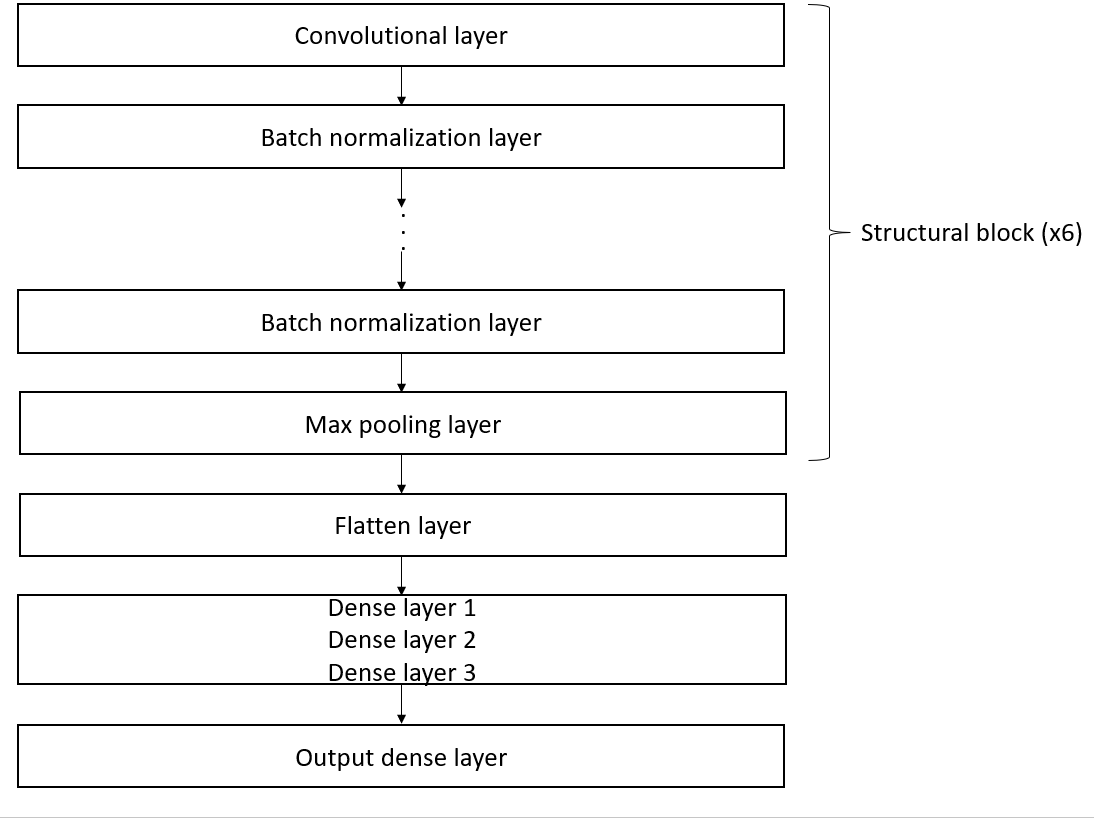
\includegraphics[width=\textwidth]{C15D3net_Architecture.png}
\end{subfigure}
\caption{Αρχικτετονική C15D3net}
\label{C15D3net_Architecture_fig}
\end{figure}

\begin{figure}[H]
\centering
\begin{subfigure}[t]{0.9\textwidth}%
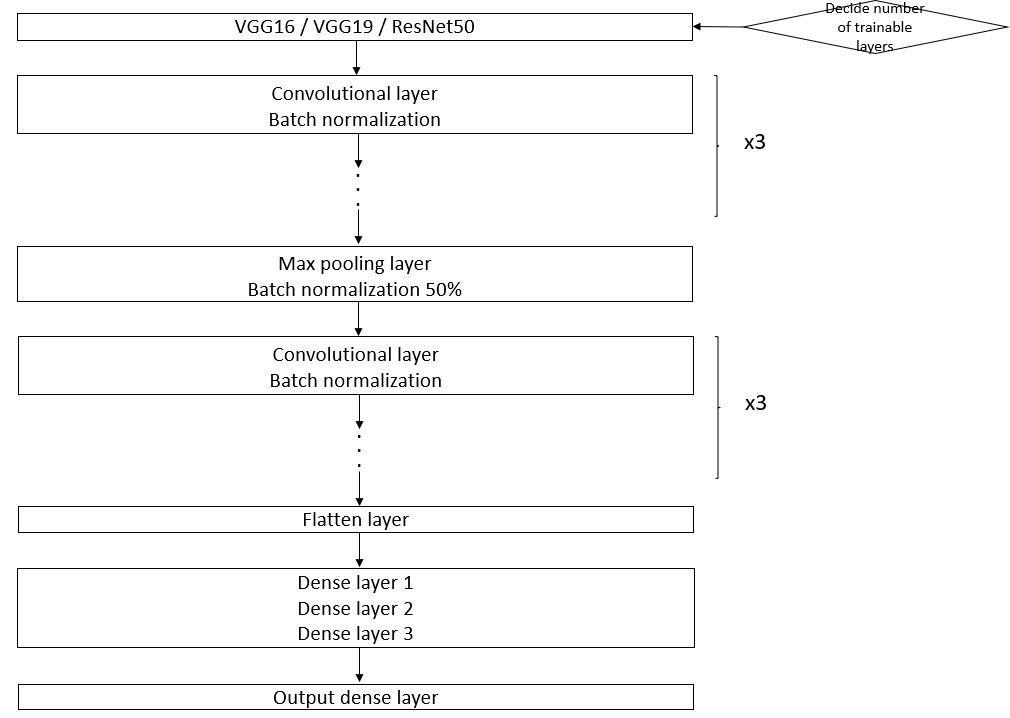
\includegraphics[width=\textwidth]{Pretrained_Architectures.png}
\end{subfigure}
\caption{Αρχικτετονικές VGG16mod, VGG19mod, ResNet50mod}
\label{Pretrained_Architectures_fig}
\end{figure}


\section{Ρύθμιση παραμέτρων}
\label{Parameters tuning}

Μετά την ανάπτυξη των διαφόρων αρχιτεκτονικών μπορεί να ακολουθήσει η διεξαγωγή δοκιμών ώστε να καταλήξουμε στο ιδανικότερο μοντέλο για την επίλυση του προβλήματος ταξινόμησης. 

Αντικειμενικός στόχος αυτών των δοκιμών ήταν η επίτευξη όσο το δυνατόν μεγαλύτερης ακρίβειας πρόβλεψης (accuracy) κατά τη διάρκεια της εκπαίδευσης, αλλά κρισιμότερα κατά την διαδικασία επαλήθευσης (validation), η οποία αποτελεί ένα καλό δείκτη της δυνατότητας γενίκευσης του αναπτυσσόμενου μοντέλου.

Έχοντας αποφασίσει, σε γενικές γραμμές, τη δομή των διαφόρων αρχιτεκτονικών, όπως παρουσιάστηκε στα σχήματα \ref{C15D3net_Architecture_fig} και \ref{Pretrained_Architectures_fig}, ακολουθεί η παρουσίαση των δοκιμών για την επιλογή της τελικής μορφής του νευρωνικού δικτύου. Οι δοκιμές αυτές μπορούν να αποδοθούν στις παρακάτω κατηγορίες.

\begin{enumerate}
\item Μέγεθος των εικόνων
\item Χρήση γεννήτριας εικόνων (image generator)
\item Χρήση regularizer L1,L2 για τη μείωση του βαθμού υπερπροσαρμογής (overfitting) στα δεδομένα
\item Επιμέρους παράμετροι εκπαίδευσης (αριθμός εποχών, είδος βελτιστοποιητή, κτλ.) για γρηγορότερη και καλύτερη σύγκλιση του μοντέλου
\item Αριθμός επιπέδων προς εκπαίδευση (trainable layers) στις αρχιτεκτονικές που χρησιμοποιούν προ-εκπαιδευμένα μοντέλα
\end{enumerate}

\begin{table}[H]
\centering
\begin{tabular}{|c|c|c|c|c|}
\hline
\diagbox{Αρχιτεκτονική}{Μέγεθος εικόνων} & (64, 64, 3) & (128, 128, 3) & (160, 160, 3) & (256, 256, 3) \\ \hline
ResNet50mod (1) & $\surd$ & $\surd$ & $\surd$ & $\surd$ \\ \hline
ResNet50mod (2) &         &         & $\surd$ &         \\ \hline
ResNet50mod (3) &         &         & $\surd$ &         \\ \hline
ResNet50mod (4) &         &         & $\surd$ &         \\ \hline
VGG16mod        &         &         & $\surd$ &         \\ \hline
VGG19mod        &         &         & $\surd$ &         \\ \hline
C15D3net        &         &         & $\surd$ &         \\ \hline
\end{tabular}
\caption{Περιπτώσεις αρχιτεκτονικών που ελέγχθηκαν}
\label{Tuning_Architectures_table}
\end{table}


Στον πίνακα \ref{Tuning_Architectures_table} παρουσιάζονται οι περιπτώσεις για τις οποίες πραγματοποιήθηκε εκτέλεση του κώδικα. Για τις αρχιτεκτονικές που παρουσιάζονται στην πρώτη στήλη του πίνακα και οι οποίες θα αναφερθούν λεπτομερέστερα παρακάτω ισχύουν τα εξής.

\begin{itemize}
\item ResNet50mod (1) : 20 προ-εκπαιδευμένα layers της ResNet50 προς εκπαίδευση, χωρίς εφαρμογή L1/L2 regularization, με χρήση γεννήτριας εικόνων
\item ResNet50mod (2) : 20 προ-εκπαιδευμένα layers της ResNet50 προς εκπαίδευση, χωρίς εφαρμογή L1/L2 regularization, χωρίς χρήση γεννήτριας εικόνων
\item ResNet50mod (3) : 20 προ-εκπαιδευμένα layers της ResNet50 προς εκπαίδευση, με χρήση L1/L2 regularization, με χρήση γεννήτριας εικόνων
\item ResNet50mod (4) : 0 προ-εκπαιδευμένα layers της ResNet50 προς εκπαίδευση, χωρίς εφαρμογή L1/L2 regularization, με χρήση γεννήτριας εικόνων
\item VGG16mod : 0 προ-εκπαιδευμένα layers της VGG16 προς εκπαίδευση, χωρίς εφαρμογή L1/L2 regularization, με χρήση γεννήτριας εικόνων
\item VGG19mod : 0 προ-εκπαιδευμένα layers της VGG19 προς εκπαίδευση, χωρίς εφαρμογή L1/L2 regularization, με χρήση γεννήτριας εικόνων
\item C15D3net : Αρχιτεκτονική που αναπτύχθηκε εξ'αρχής. Αποτελείται από 15 συνελικτικά και 3 πλήρως διασυνδεδεμένα επίπεδα 
\end{itemize}

\subsubsection{Μέγεθος εικόνων}

Αρχικά, η πρώτη παράμετρος που πρέπει να καθοριστεί είναι το μέγεθος των εικόνων που θα χρησιμοποιηθούν κατά την εκπαίδευση. Πρόκειται για μια πολύ σημαντική παράμετρο της οποίας η τιμή επιλέγεται πριν αρχίσει η διαδικασία εκπαίδευσης, κατά το στάδιο της προ-επεξεργασίας εικόνων, αλλά έχει σημαντικές συνέπειες για την πολυπλοκότητα, την τελική ακρίβεια του μοντέλου αλλά και τη δυνατότητα εκπαίδευσης του μοντέλου λόγω επάρκειας μνήμης όπως και τον χρόνο εκπαίδευσης. 

Στο σχήμα \ref{image_compare_sizes_training} φαίνεται η ακρίβεια που επιτυγχάνεται κατά τη διάρκεια εκπαίδευσης για την ίδια ακριβώς αρχιτεκτονική, η οποία είναι η τροποποιημένη ResNet50 με 20 trainable layers και χωρίς τη χρήση regularizer, δηλαδή η περίπτωση ResNet50mod (1) που αναφέραμε πιο πάνω, για τέσσερις διαφορετικές διαστάσεις εικόνων (64, 64, 3) (128, 128, 3), (160, 160, 3) και (256, 256, 3).


Στο σχήμα \ref{image_compare_sizes_validation}, φαίνονται οι τιμές κατά την διαδικασία της επαλήθευσης. Επιπλέον στον πίνακα \ref{Different_sizes_same_architecture_table} παρουσιάζεται συγκεντρωτικά ο αριθμός των παραμέτρων προς εκπαίδευση για κάθε μια από αυτές τις περιπτώσεις, αλλά και για όλες τις υπόλοιπες περιπτώσεις τις οποίες μελετήσαμε.

\begin{figure}[H]
\centering
\begin{subfigure}[t]{0.49\textwidth}
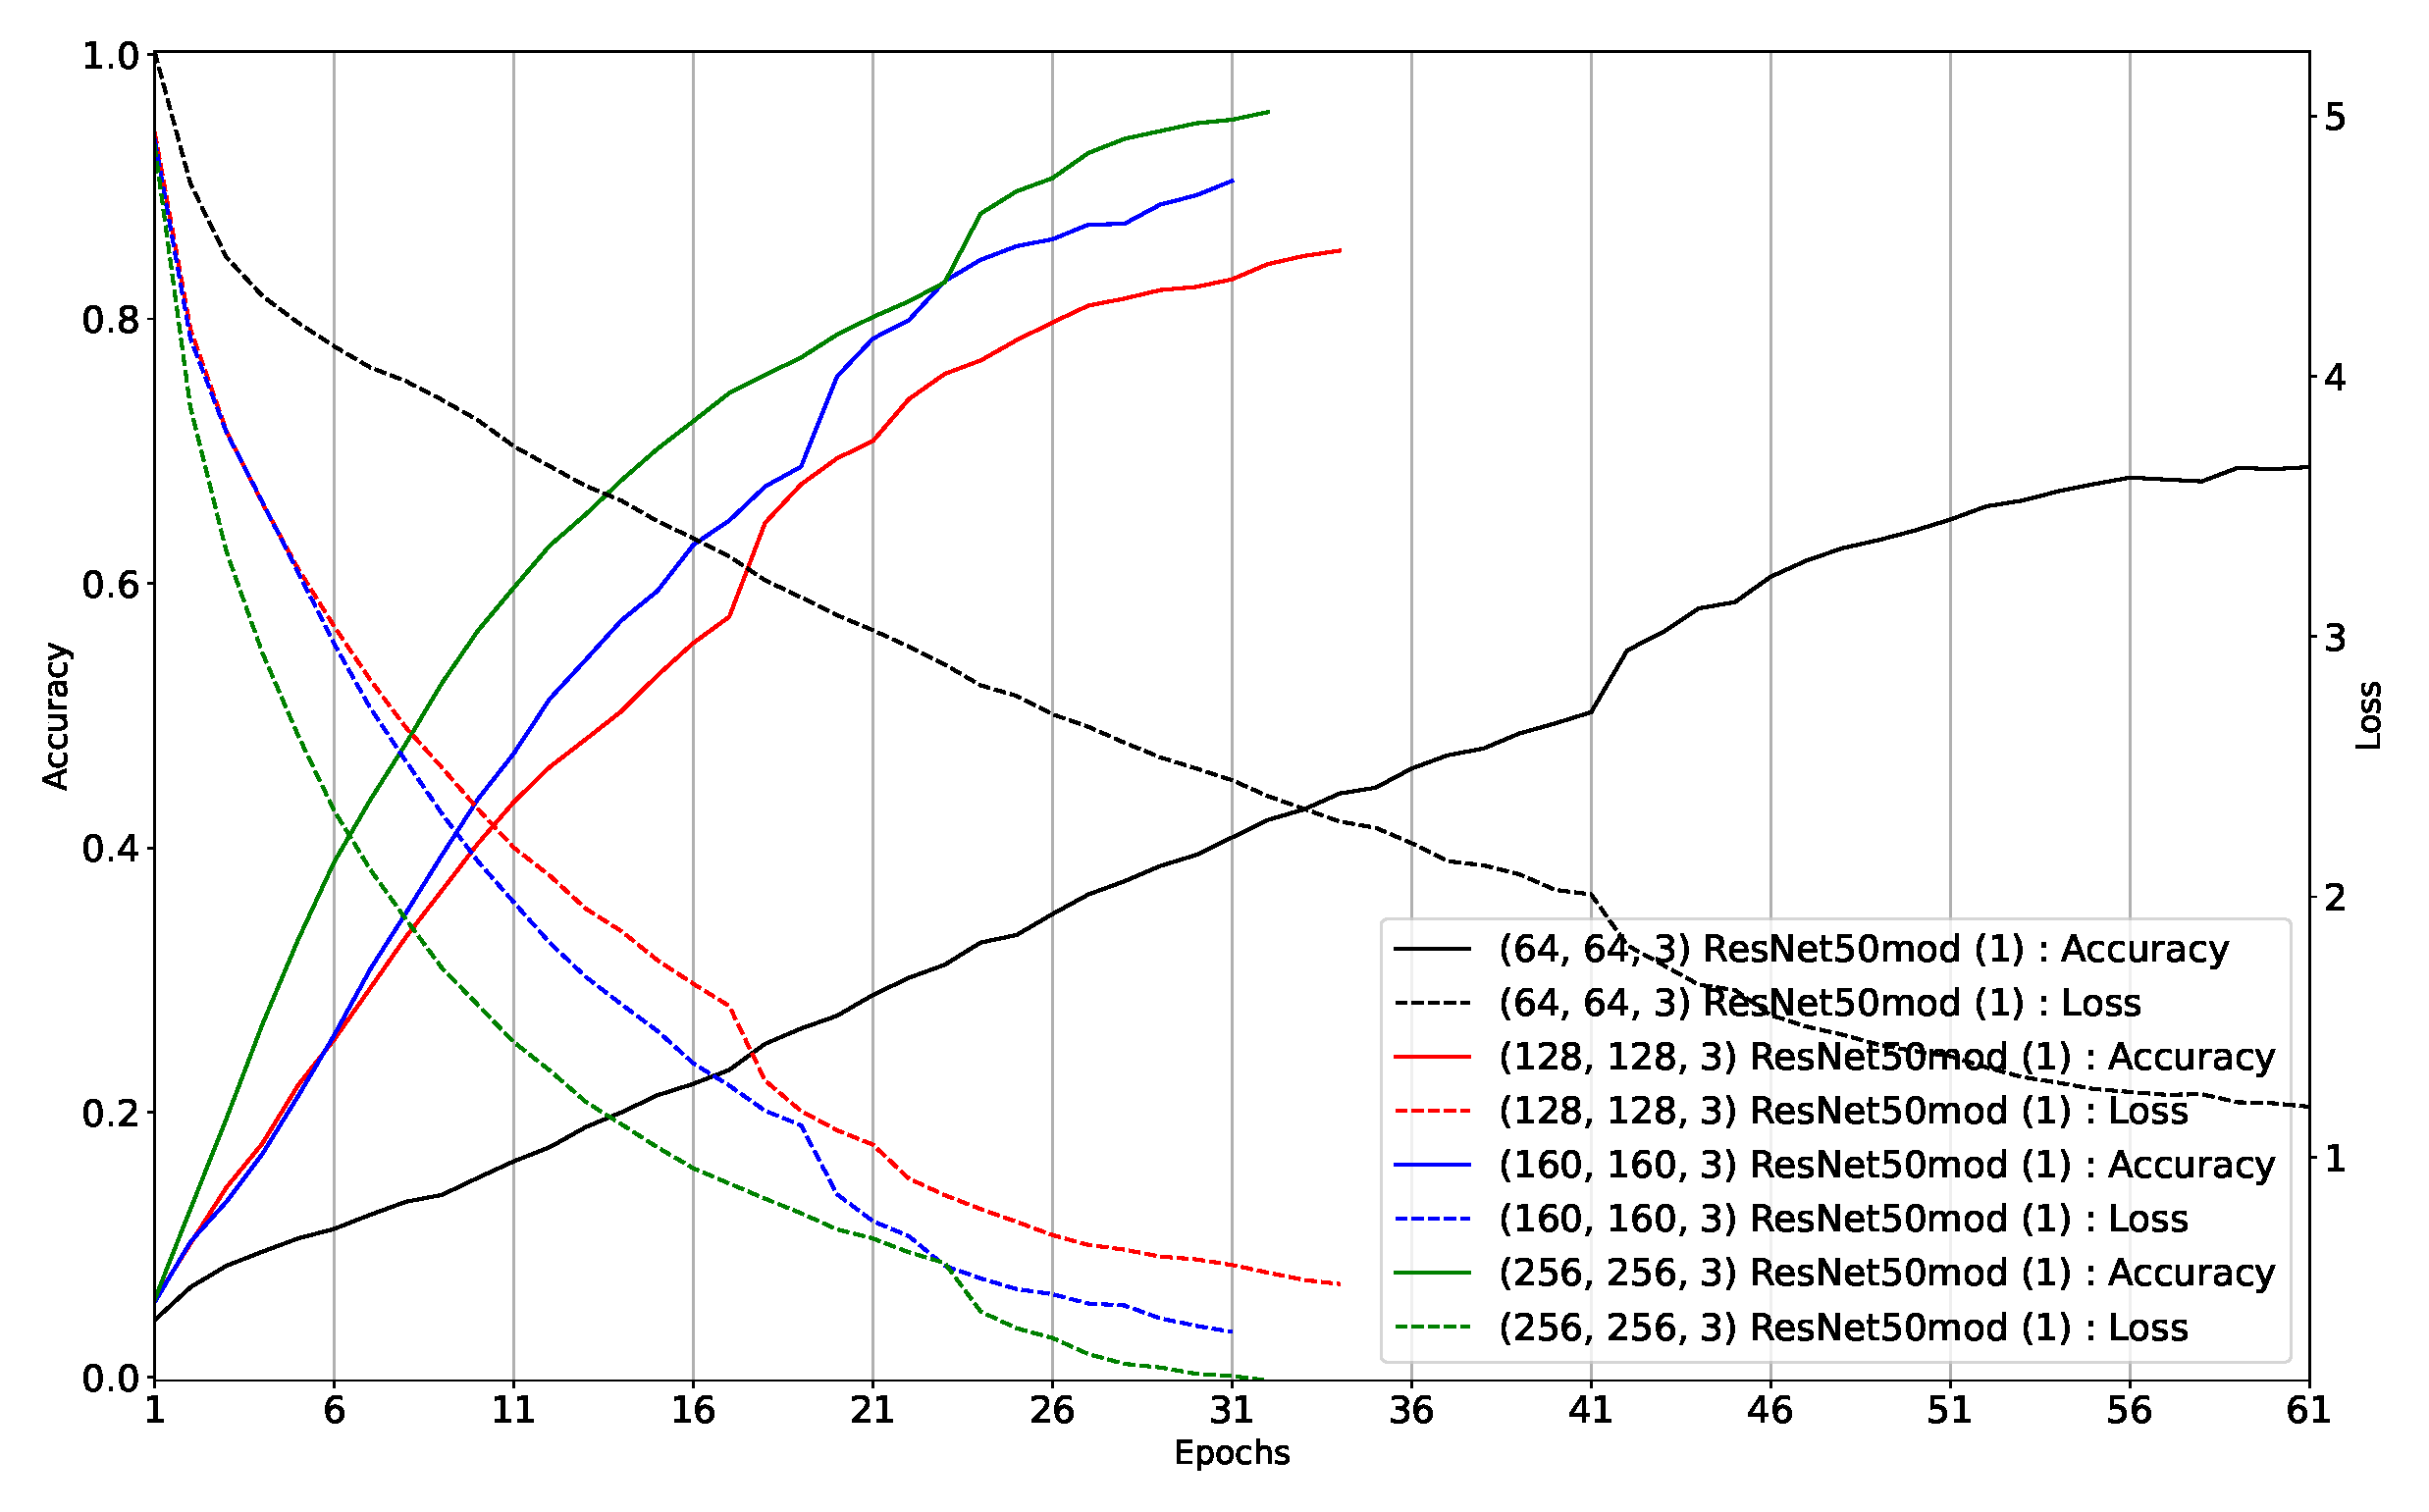
\includegraphics[width=\textwidth]{History_Compare_Sizes_Training.pdf}
\caption{Training}
\label{image_compare_sizes_training}
\end{subfigure}
\begin{subfigure}[t]{0.49\textwidth}
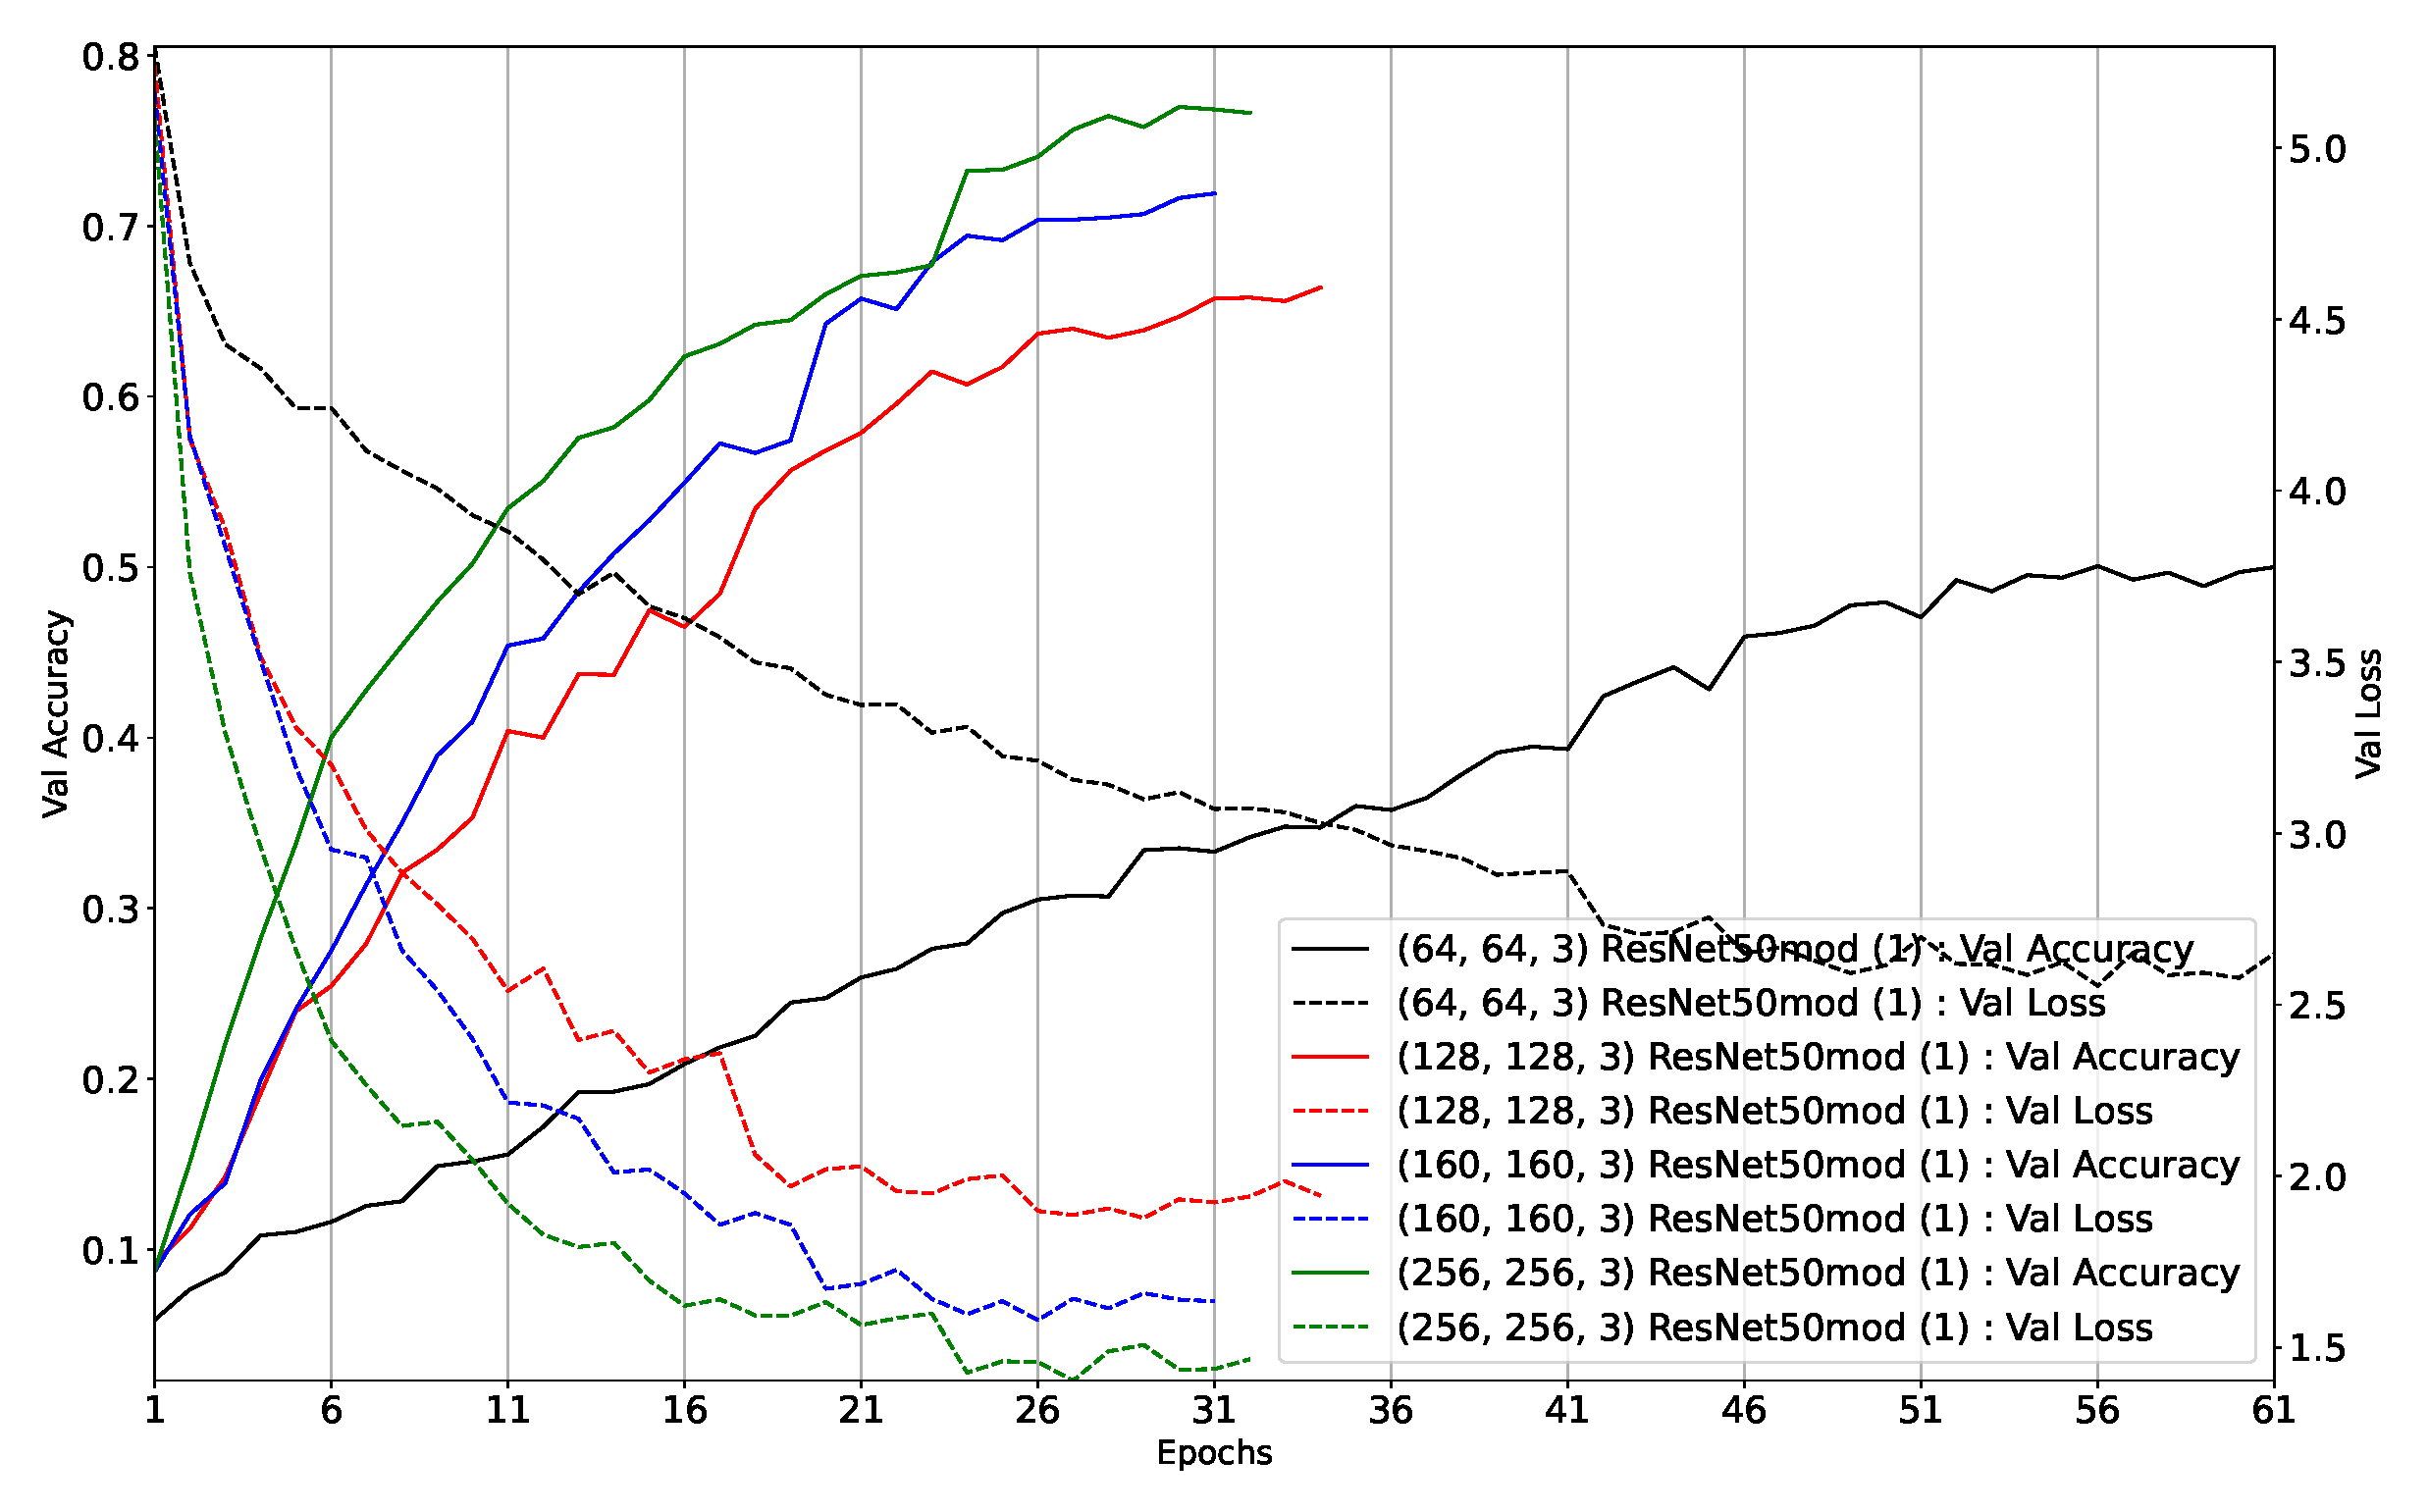
\includegraphics[width=\textwidth]{History_Compare_Sizes_Validation.pdf}
\caption{Validation}
\label{image_compare_sizes_validation}
\end{subfigure}
\caption{Επίδραση μεγέθους εικόνας}
\label{Different_sizes_same_architecture_fig}
\end{figure}

\begin{table}[H]
\centering
\begin{tabular}{|c|c|c|c|c|}
\hline
\diagbox{Αρχιτεκτονική}{Μέγεθος εικόνων}  & (64, 64, 3) & (128, 128, 3) & (160, 160, 3) & (256, 256, 3) \\ \hline
ResNet50mod (1) & 30,221,728 & 30,477,888 & 30,561,424 & 32,403,328  \\ \hline
ResNet50mod (2) &            &            & 30,561,424 &             \\ \hline
ResNet50mod (3) &            &            & 30,561,424 &             \\ \hline
ResNet50mod (4) &            &            & 21,630,096 &             \\ \hline
VGG16mod        &            &            & 7,423,621  &             \\ \hline
VGG19mod        &            &            & 7,423,621  &             \\ \hline
C15D3net        &            &            & 6,114,716  &             \\ \hline
\end{tabular}
\caption{Αριθμός παραμέτρων προς εκπαίδευση}
\label{Different_sizes_same_architecture_table}
\end{table}

Όπως είναι φανερό από τον πίνακα \ref{Different_sizes_same_architecture_table} η χρήση μεγαλύτερων σε μέγεθος εικόνων δεν αυξάνει ιδιαίτερα τον αριθμό των προς εκπαίδευση παραμέτρων, αλλά το σχήμα \ref{Different_sizes_same_architecture_fig} καταδεικνύει ότι η ακρίβεια που επιτυγχάνει το μοντέλο τόσο κατά την εκπαίδευση όσο και κατά την επαλήθευση βελτιώνεται με την αύξηση του μεγέθους, ενώ αντίθετα η συνάρτηση κόστους βαίνει διαρκώς μειούμενη. Αυτό μπορεί να εξηγηθεί από το γεγονός ότι οι μεγαλύτερες σε μέγεθος εικόνες περιέχουν περισσότερες λεπτομέρειες οι οποίες μπορούν να εντοπιστούν κατά την εκπαίδευση του νευρωνικού δικτύου.

Από την παραπάνω ανάλυση θα περίμενε κανείς να επιλεγούν για την συνέχεια των δοκιμών η χρήση εικόνων (256, 256, 3). Όμως για την σύγκριση μεταξύ μοντέλων αρκεί να έχουν εκπαιδευτεί όλα με τον ίδιο μέγεθος εικόνων οπότε και προτιμήθηκε οι υπόλοιπες δοκιμές να γίνουν με εικόνες διαστάσεων (160, 160, 3).

\subsubsection{Γεννήτρια εικόνων}

Ένα άλλο πολύ σημαντικό στοιχείο για την αποτελεσματική εκπαίδευση του νευρωνικού δικτύου είναι η χρήση γεννήτριας εικόνων (image generator). Πρόκειται επί της ουσίας για μια συνάρτηση βιβλιοθήκης της python η οποία πραγματοποιεί αλλαγές στις εικόνες που χρησιμοποιούνται κατά την εκπαίδευση αλλά και την επαλήθευση. Λόγω της διαφοροποίησης των εικόνων εισόδου, αναμένεται μείωση του βαθμού υπερπροσαρμογής αλλά και αυξημένη ακρίβεια πρόβλεψης, το οποίο επιβεβαιώνεται στο σχήμα \ref{image_generator_fig}. 

Πιο αναλυτικά στο σχήμα \ref{image_generator_training} το οποίο αναπαριστά την εξέλιξη των τιμών της ακρίβειας και της συνάρτησης κόστους κατά την εκπαίδευση, βλέπουμε ότι και στις δύο περιπτώσεις, με και χωρίς τη χρήση γεννήτριας αριθμών τα αποτελέσματα, είναι παραπλήσια. Το ενδιαφέρον στοιχείο όμως εμφανίζεται από την παρατήρηση του σχήματος \ref{image_generator_validation}, όπου όπως και προηγουμένως παρουσιάζεται η ιστορία εξέλιξης της ακρίβειας και της συνάρτησης κόστους για το σύνολο δεδομένων επαλήθευσης. Γίνεται εμφανές παρατηρώντας τις μαύρες καμπύλες, ότι σχετικά γρήγορα κατά τη διάρκεια της εκπαίδευσης χωρίς τη χρήση γεννήτριας εικόνων, το μοντέλο οδηγείται σε υπερπροσαρμογή, καθώς η συνάρτηση κόστους αυξάνει την τιμή και αντίστοιχα η επιτυγχανόμενη ακρίβεια είναι πολύ μικρότερη της ακρίβειας του μοντέλου με χρήση image generator. 

Τέλος, στον πίνακα \ref{image_generator_table} φαίνονται τα όρια των επιτρεπόμενων αλλαγών στις εικόνες. Αυτά επιλέχθηκαν με χρήση πολύ λίγων επαναλήψεων και πιθανώς μια συστηματικότερη εξέταση των δυνατών τιμών τους να οδηγούσε σε μικρή βελτίωση των αποτελεσμάτων.


\begin{figure}[H]
\centering
\begin{subfigure}[t]{0.49\textwidth}
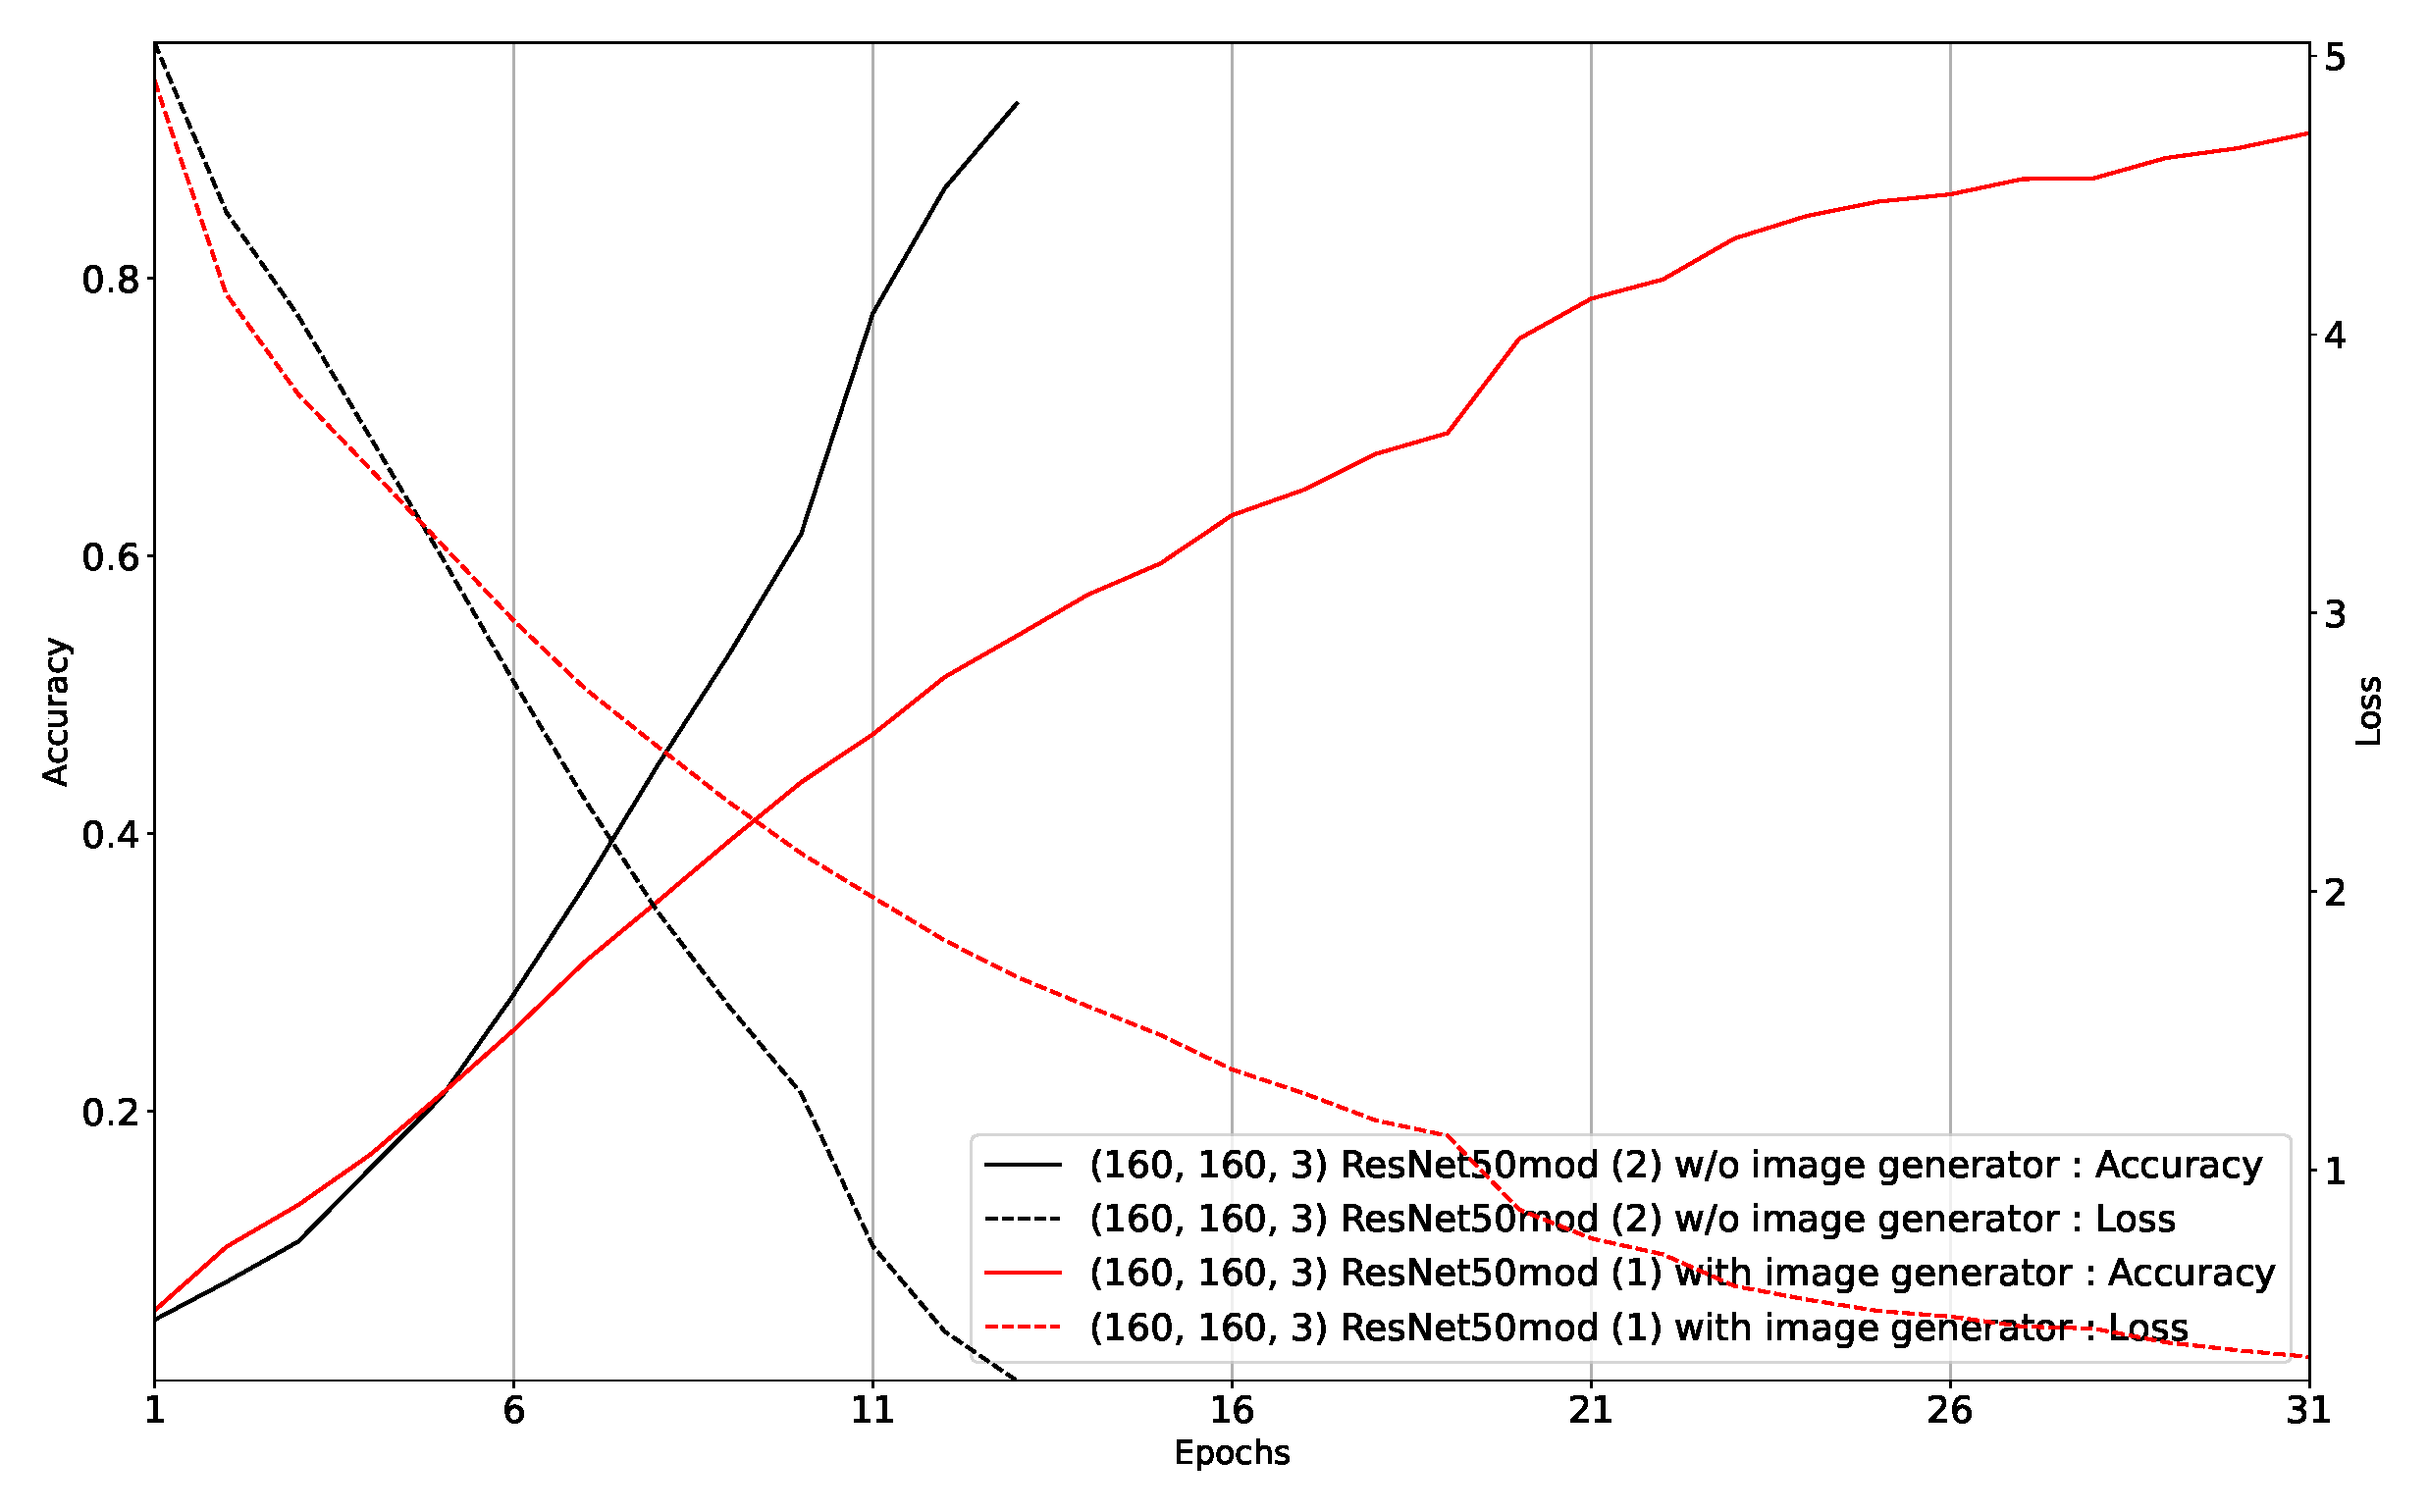
\includegraphics[width=\textwidth]{History_Compare_Generators_Training.pdf}
\caption{Training}
\label{image_generator_training}
\end{subfigure}
\begin{subfigure}[t]{0.49\textwidth}
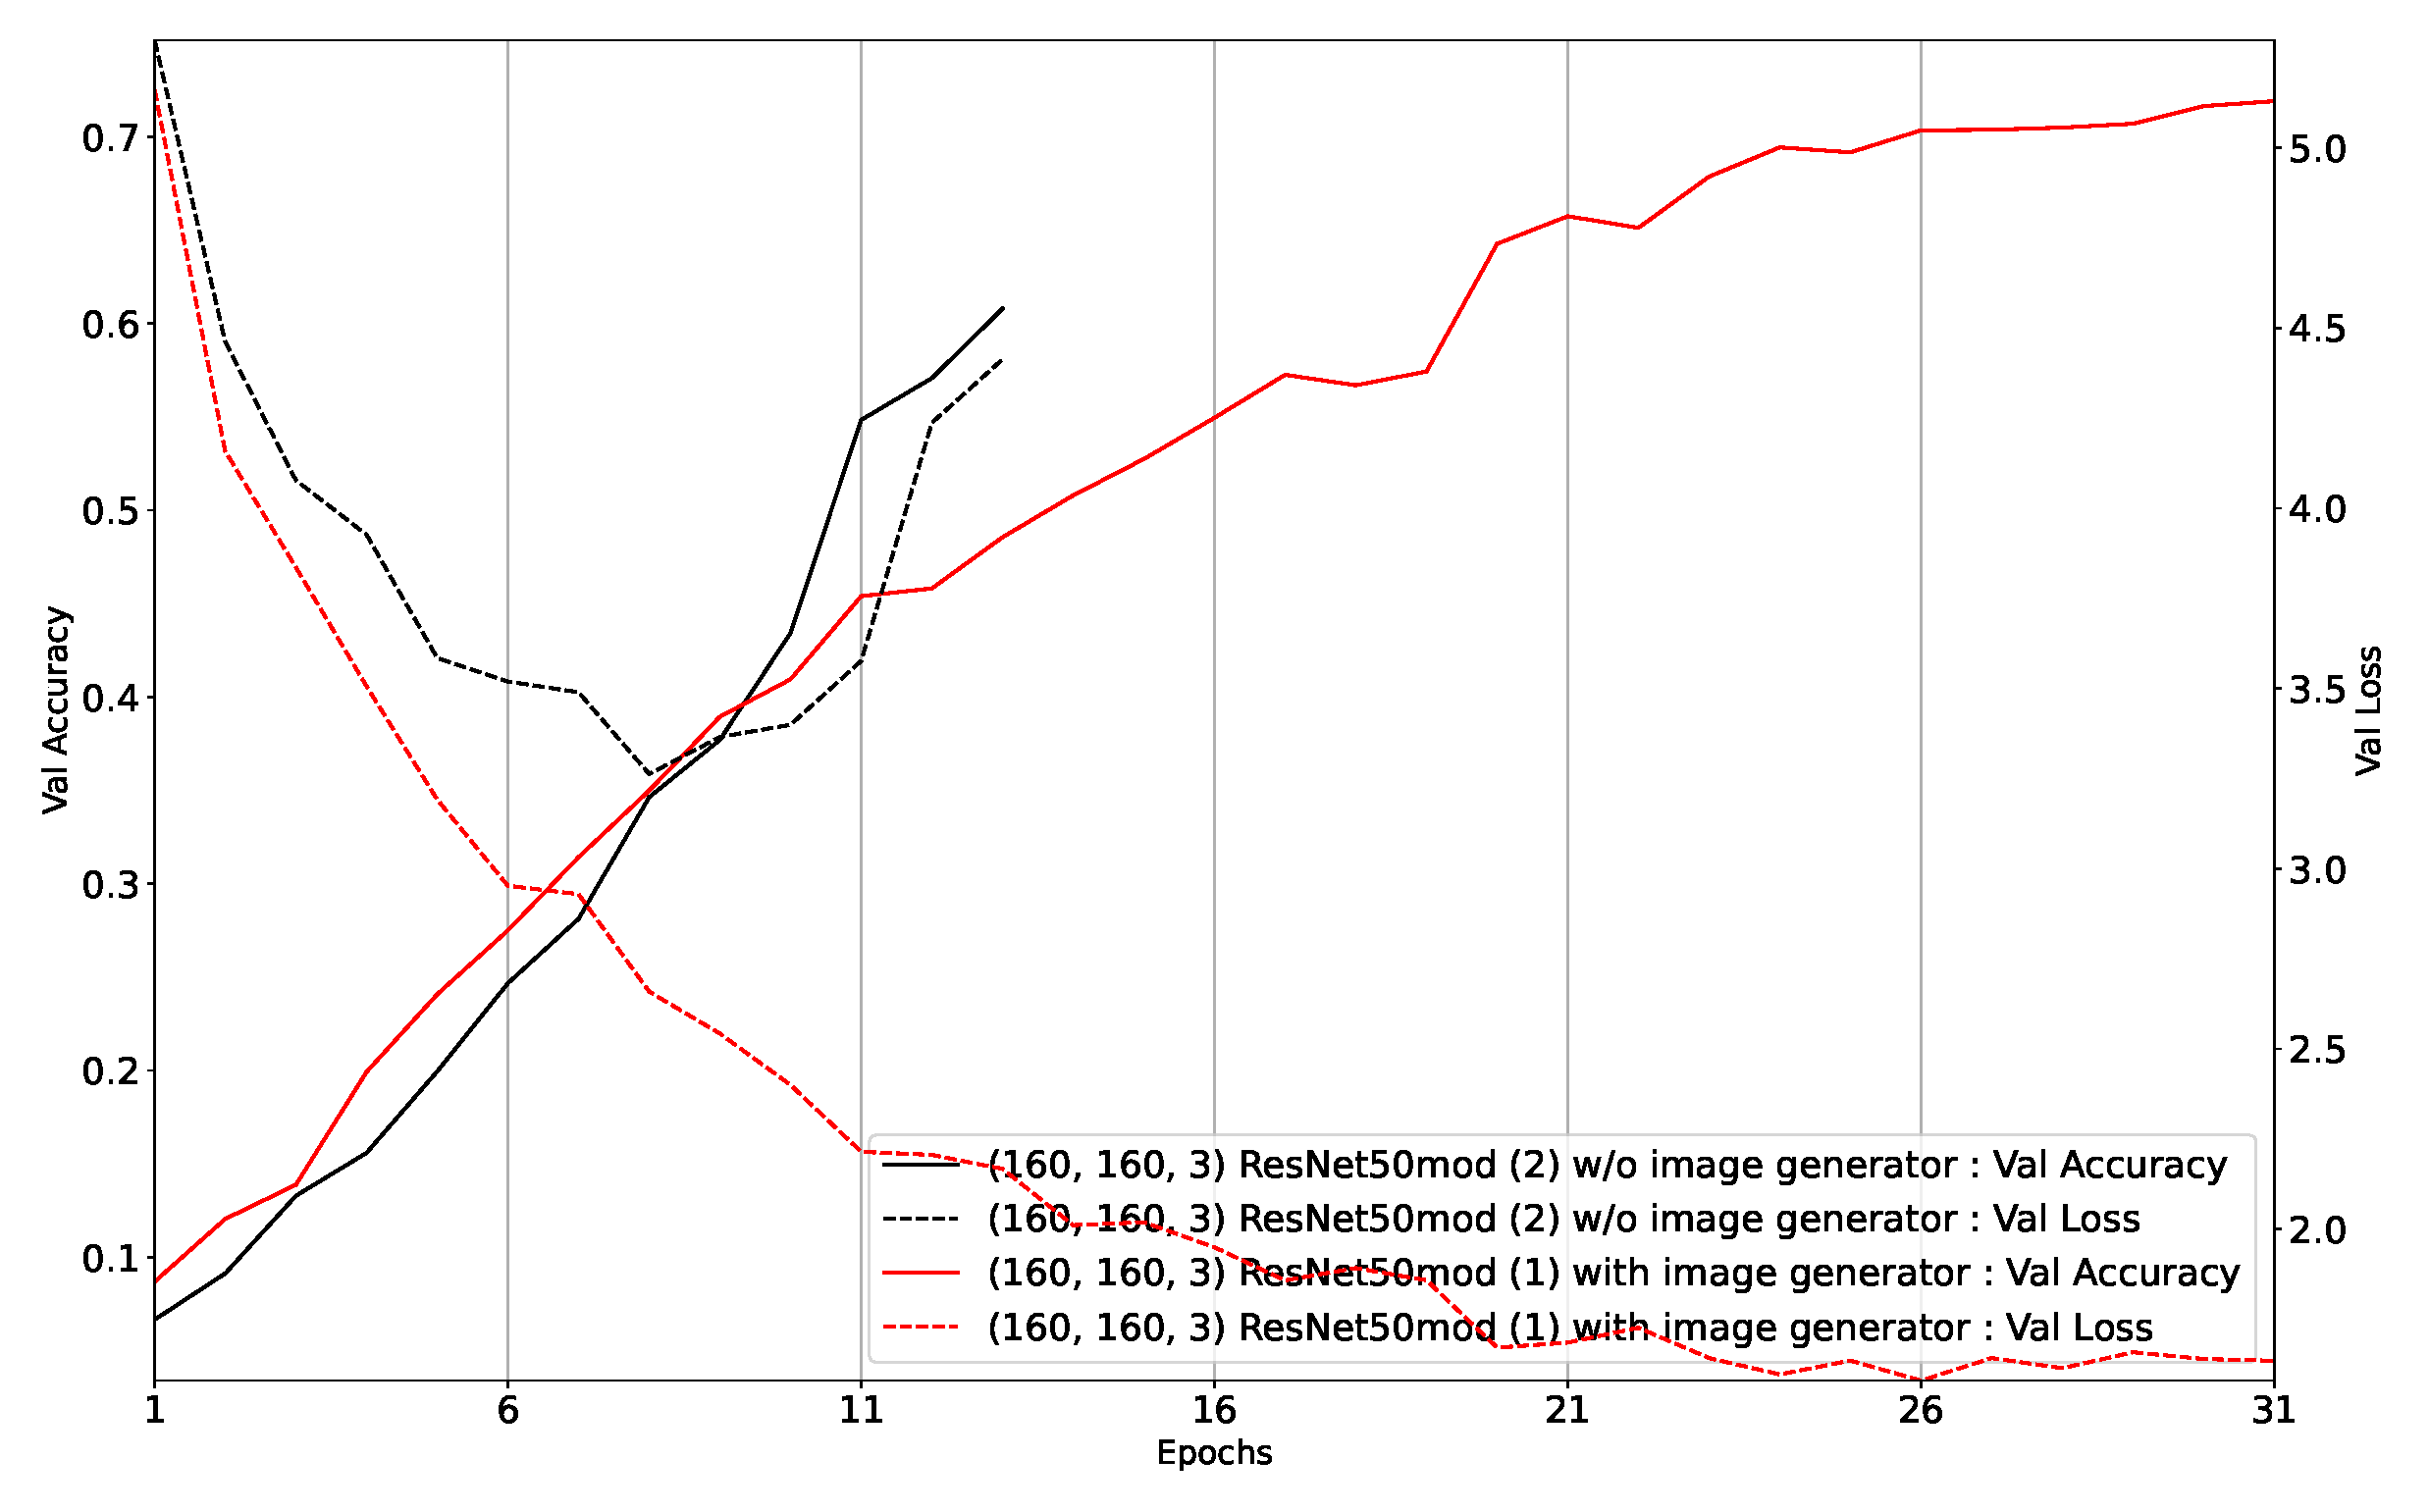
\includegraphics[width=\textwidth]{History_Compare_Generators_Validation.pdf}
\caption{Validation}
\label{image_generator_validation}
\end{subfigure}
\caption{Επίδραση χρήσης γεννήτριας εικόνων}
\label{image_generator_fig}
\end{figure}


\begin{table}[H]
\centering
\begin{tabular}{|c|c|}
\hline
Παράμετρος           & Τιμή           \\ \hline
rotation\_range      & 30             \\ \hline
width\_shift\_range  & 0.1            \\ \hline
height\_shift\_range & 0.1            \\ \hline
brightness\_range    & {[}0.5, 1.0{]} \\ \hline
shear\_range         & 0.2            \\ \hline
zoom\_range          & 0.2            \\ \hline
horizontal\_flip     & True           \\ \hline
\end{tabular}
\caption{Παράμετροι image generator}
\label{image_generator_table}
\end{table}

\subsubsection{Κανονικοποίηση (Regularization)}

Μια άλλη σημαντική δοκιμή αφορά την χρήση της κανονικοποίησης των δεδομένων, μέσω της οποίας δύναται να μειωθεί η επίδραση της υπερπροσαρμογής στα νευρωνικά δίκτυα. Λόγω του μεγάλου αριθμού των παραμέτρων προς εκπαίδευση τα νευρωνικά δίκτυα έχουν την τάση να οδηγούνται σε υπερπροσαρμογή.  Ο τρόπος με τον οποίο επιτυγχάνεται αυτό στην παρούσα εργασία είναι μέσω της χρήσης επιπέδων απόρριψης (dropout layer) και την κανονικοποίηση L1 και L2. 

Σχετικά με τα dropout layers αυτά λειτουργούν με τον ακόλουθο τρόπο. Κατά τη διάρκεια της εκπαίδευσης και πιο συγκεκριμένα κατά το βήμα της προώθησης προς τα εμπρός (forward propagation) ορισμένοι από τους νευρώνες του δικτύου απενεργοποιούνται. Έτσι το δίκτυο πρέπει να εξαρτηθεί από άλλους ενεργούς νευρώνες για την αποτελεσματικότερη μάθηση. Πρόκειται δηλαδή για μια μεθοδολογία η οποία χρησιμοποιείται για να μειώσει την ευαισθησία του μοντέλου σε συγκεκριμένα χαρακτηριστικά και να βελτιώσει τη γενίκευση του μοντέλου. 

Στην παρούσα αναφορά δεν φαίνονται οι δοκιμές που έγιναν για τον αριθμό των dropout layers αλλά και το ποσοστό των νευρώνων που απορρίπτονται. Παρόλα αυτά σε όλες τις αρχιτεκτονικές του σχήματος \ref{Pretrained_Architectures_fig} χρησιμοποιήθηκε ένα dropout layer με 50\% ποσοστό απόρριψης.

Οι μέθοδοι κανονικοποίησης L1 και L2 εισάγουν έναν όρο κανονικοποίησης στη συνάρτηση κόστους του μοντέλου, το οποίο οδηγεί σε μηδενισμό ή μείωση της τιμής κάποιων εκ των παραμέτρων του μοντέλου με αποτέλεσμα να μειώνεται η υπερπροσαρμογή του μοντέλου. 

Στο σχήμα \ref{Different_regularizer_same_architecture_fig} παρουσιάζεται η επίδραση που έχει στην ακρίβεια του μοντέλου η χρήση της κανονικοποίησης. Όπως φαίνεται η εφαρμογή που επιχειρήθηκε δεν είχε κάποιο θετικό αποτέλεσμα, καθώς φαίνεται να οδηγεί σε μικρή σχετικά υποπροσαρμογή το μοντέλο και επιπλέον να οδηγεί το μοντέλο σε περισσότερες επαναλήψεις έως ότου συγκλίνει. 

Για αυτό τον λόγο δεν επιλέχθηκε η χρήση L1, L2 regularizer στις υπόλοιπες δοκιμές και στο τελικό μοντέλο. 

\begin{figure}[H]
\centering
\begin{subfigure}[t]{0.49\textwidth}
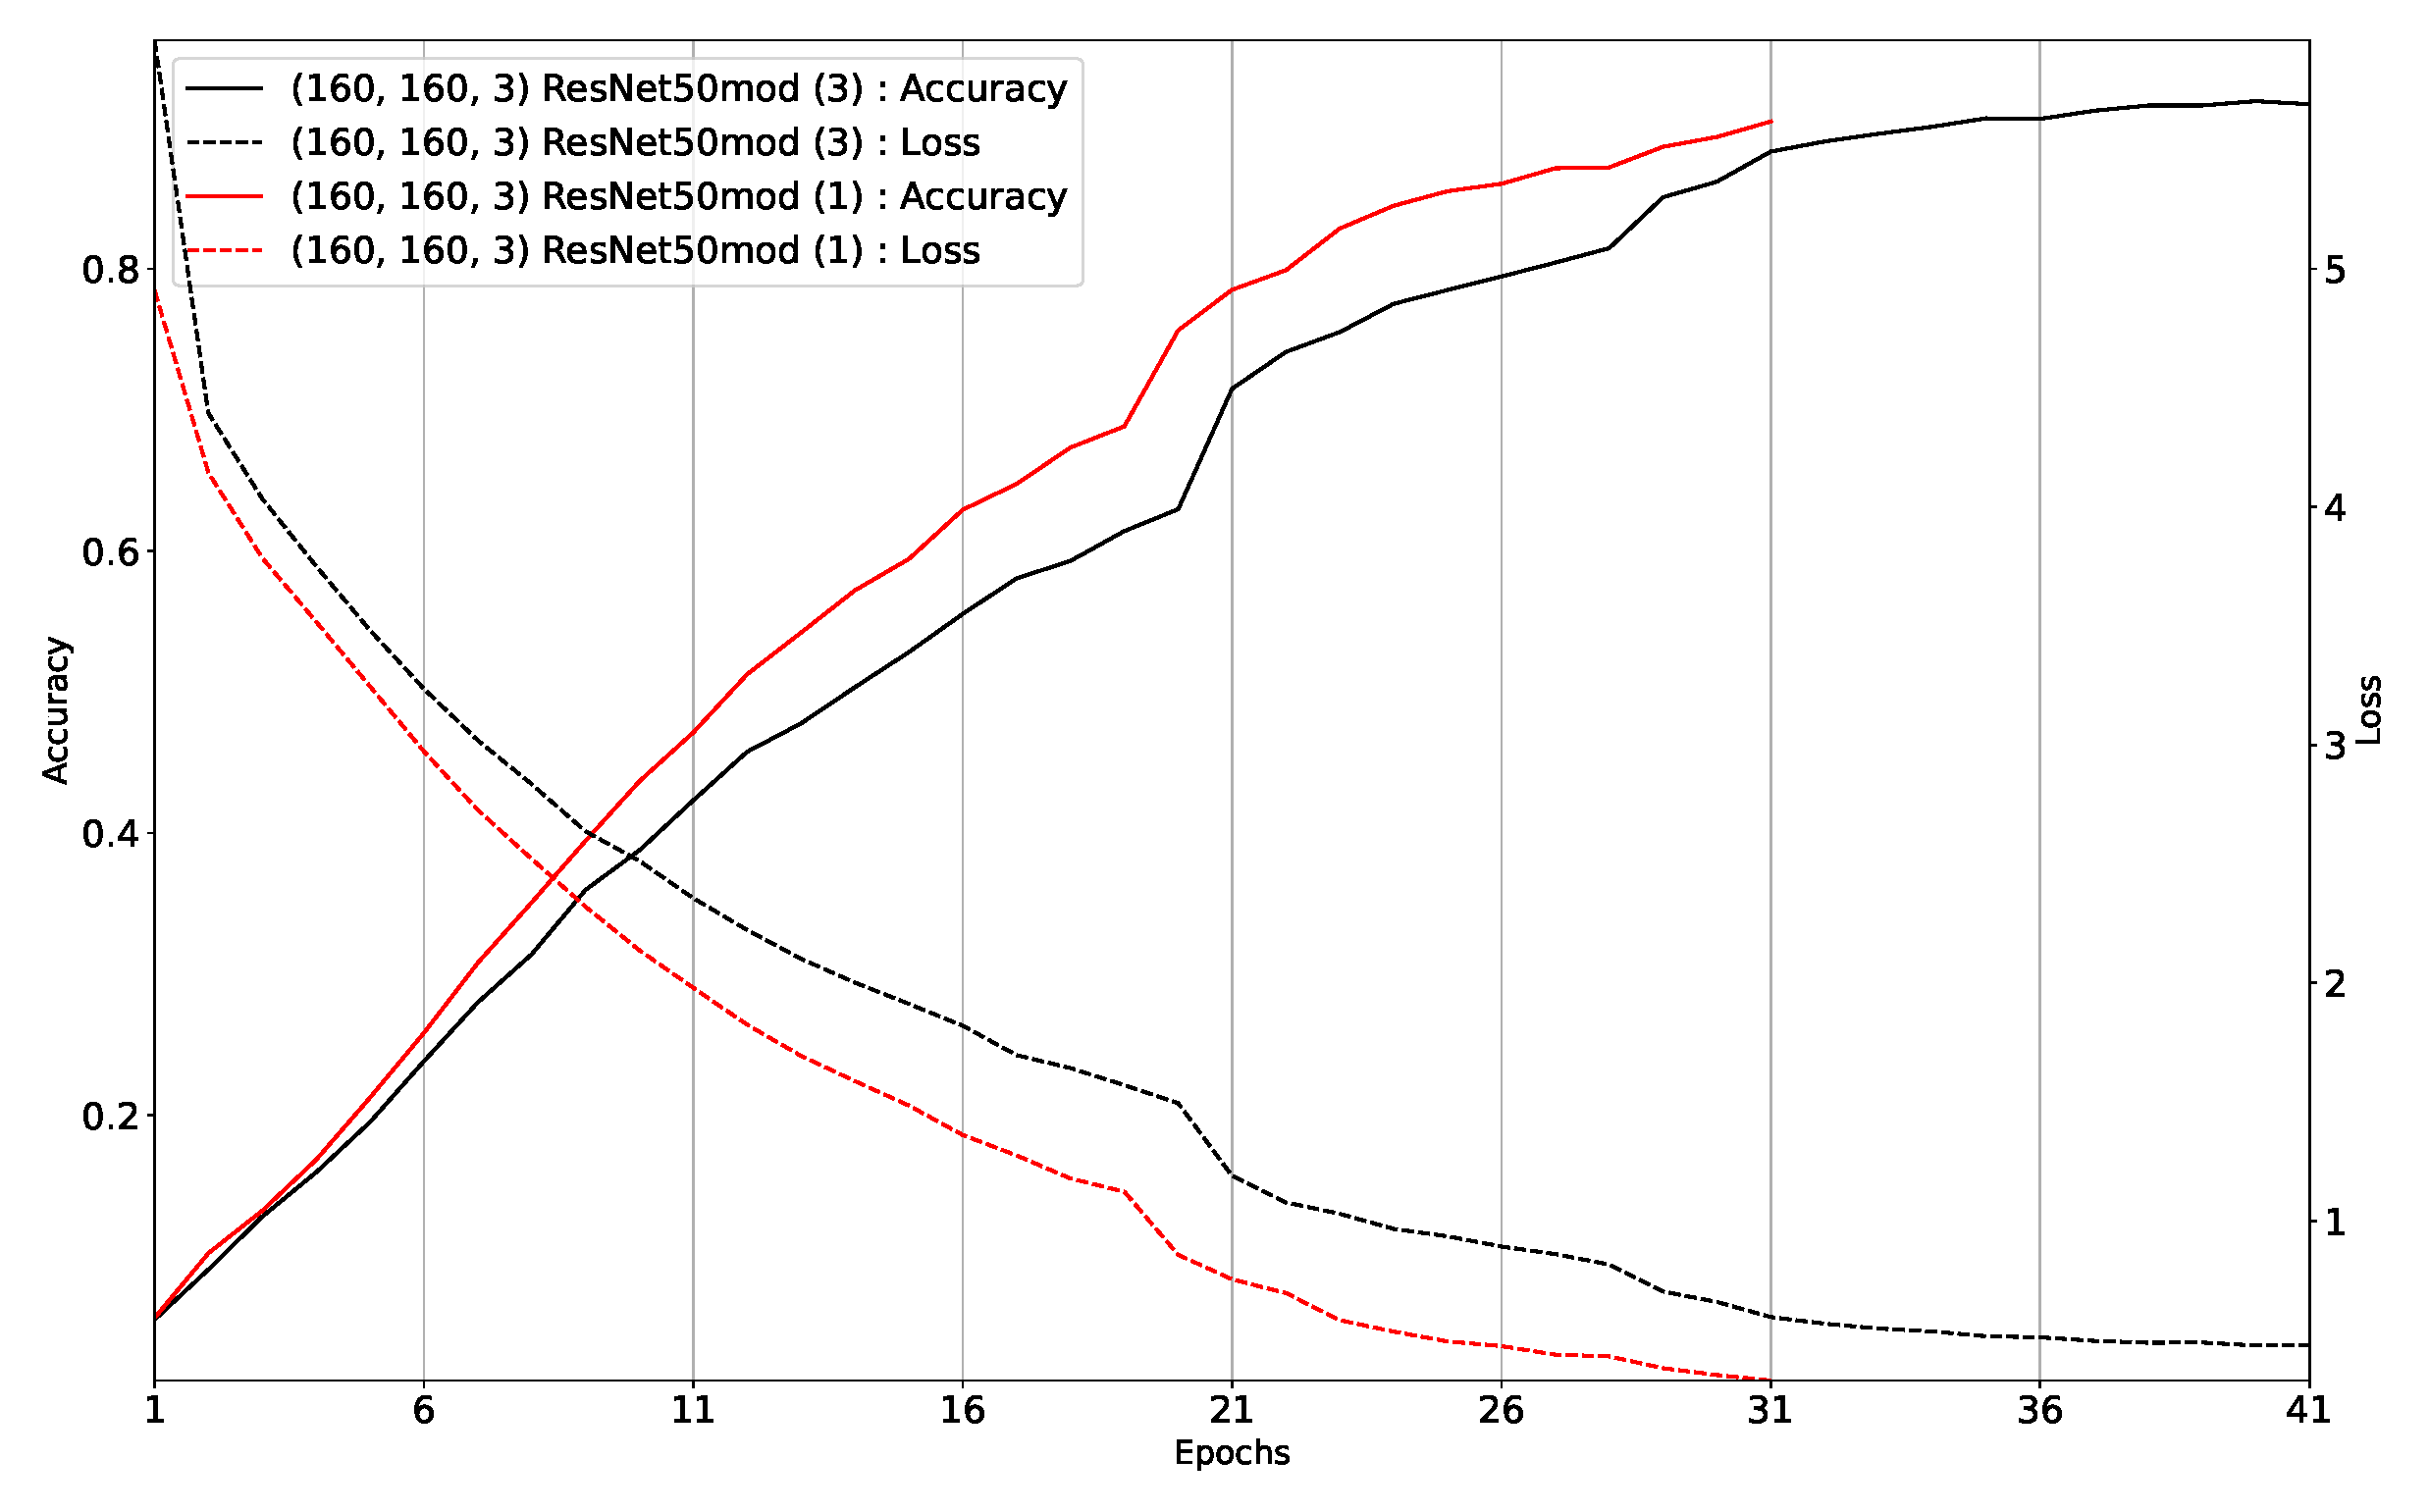
\includegraphics[width=\textwidth]{History_Compare_Regularizers_Training.pdf}
\caption{Training}
\label{image_regularizers_training}
\end{subfigure}
\begin{subfigure}[t]{0.49\textwidth}
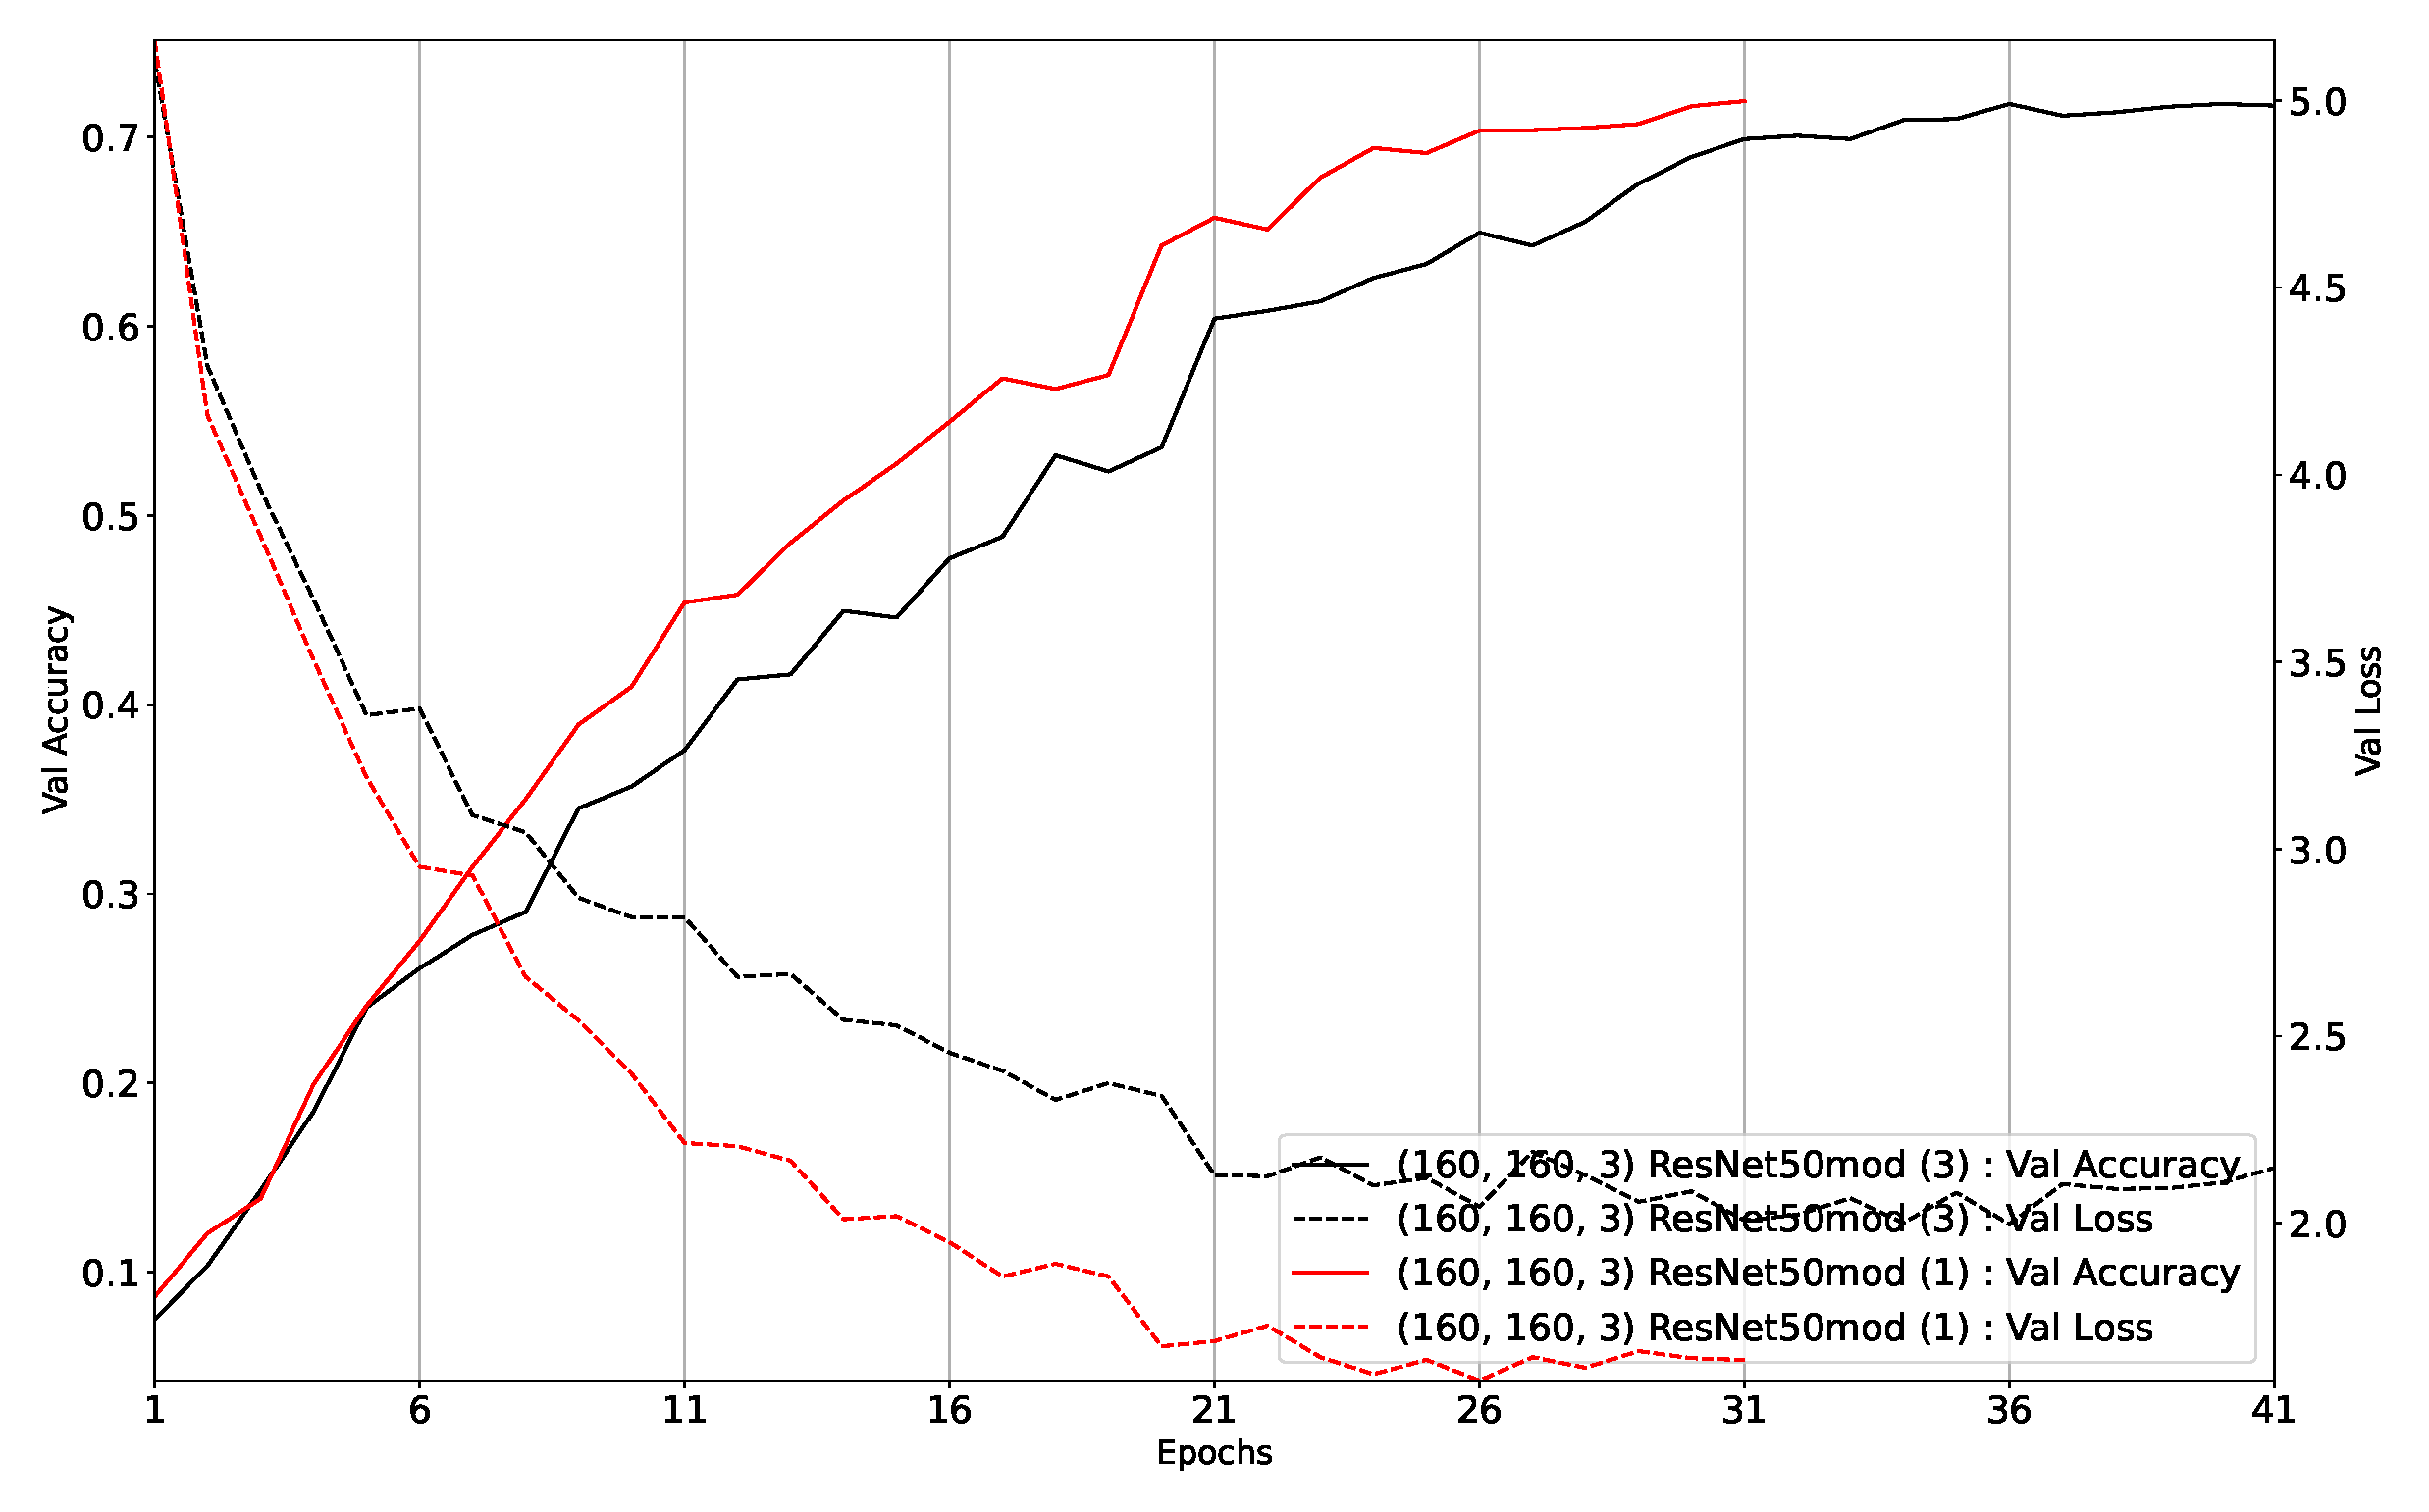
\includegraphics[width=\textwidth]{History_Compare_Regularizers_Validation.pdf}
\caption{Validation}
\label{image_regularizers_validation}
\end{subfigure}
\caption{Επίδραση χρήσης regularizer}
\label{Different_regularizer_same_architecture_fig}
\end{figure}

\subsubsection{Επιμέρους παράμετροι \& αριθμός επιπέδων προς εκπαίδευση}
Η χρήση διαφορετικών βελτιστοποιητών βρέθηκε πως δεν έχει σημαντική επίδραση στο τελικό αποτέλεσμα, αντίθετα με τον ρυθμό μάθησης (learning rate) και πιο συγκεκριμένα τον τρόπο με τον οποίο αυτός μειώνεται όταν το validation loss σταματάει να βελτιώνεται με το πέρασμα των εποχών εκπαίδευσης. 

Για να αυξήσουμε όσο το δυνατόν περισσότερο την ακρίβεια πρόβλεψης δοκιμάστηκε το ξεπάγωμα κάποιων επιπέδων στο προ-εκπαιδευμένο δίκτυο. Πρόκειται δηλαδή για την περίπτωση ResNet50mod (4), όπως αυτή αναφέρεται στους πίνακες \ref{Tuning_Architectures_table} και \ref{Different_sizes_same_architecture_table}. Στην περίπτωση του ξεπαγώματος επιπέδων όπως φαίνεται και στο σχήμα \ref{Unfreeze_Layers_fig} η αύξηση των επιπέδων προς εκπαίδευση οδηγεί σε βελτίωση της ακρίβειας το οποίο είναι αναμενόμενο από τη στιγμή που υπάρχουν περισσότερες προς εκπαίδευση παράμετροι. Πρόκειται για τη λογική που χρησιμοποιείται στο transfer learning.

\begin{figure}[H]
\centering
\begin{subfigure}[t]{0.49\textwidth}
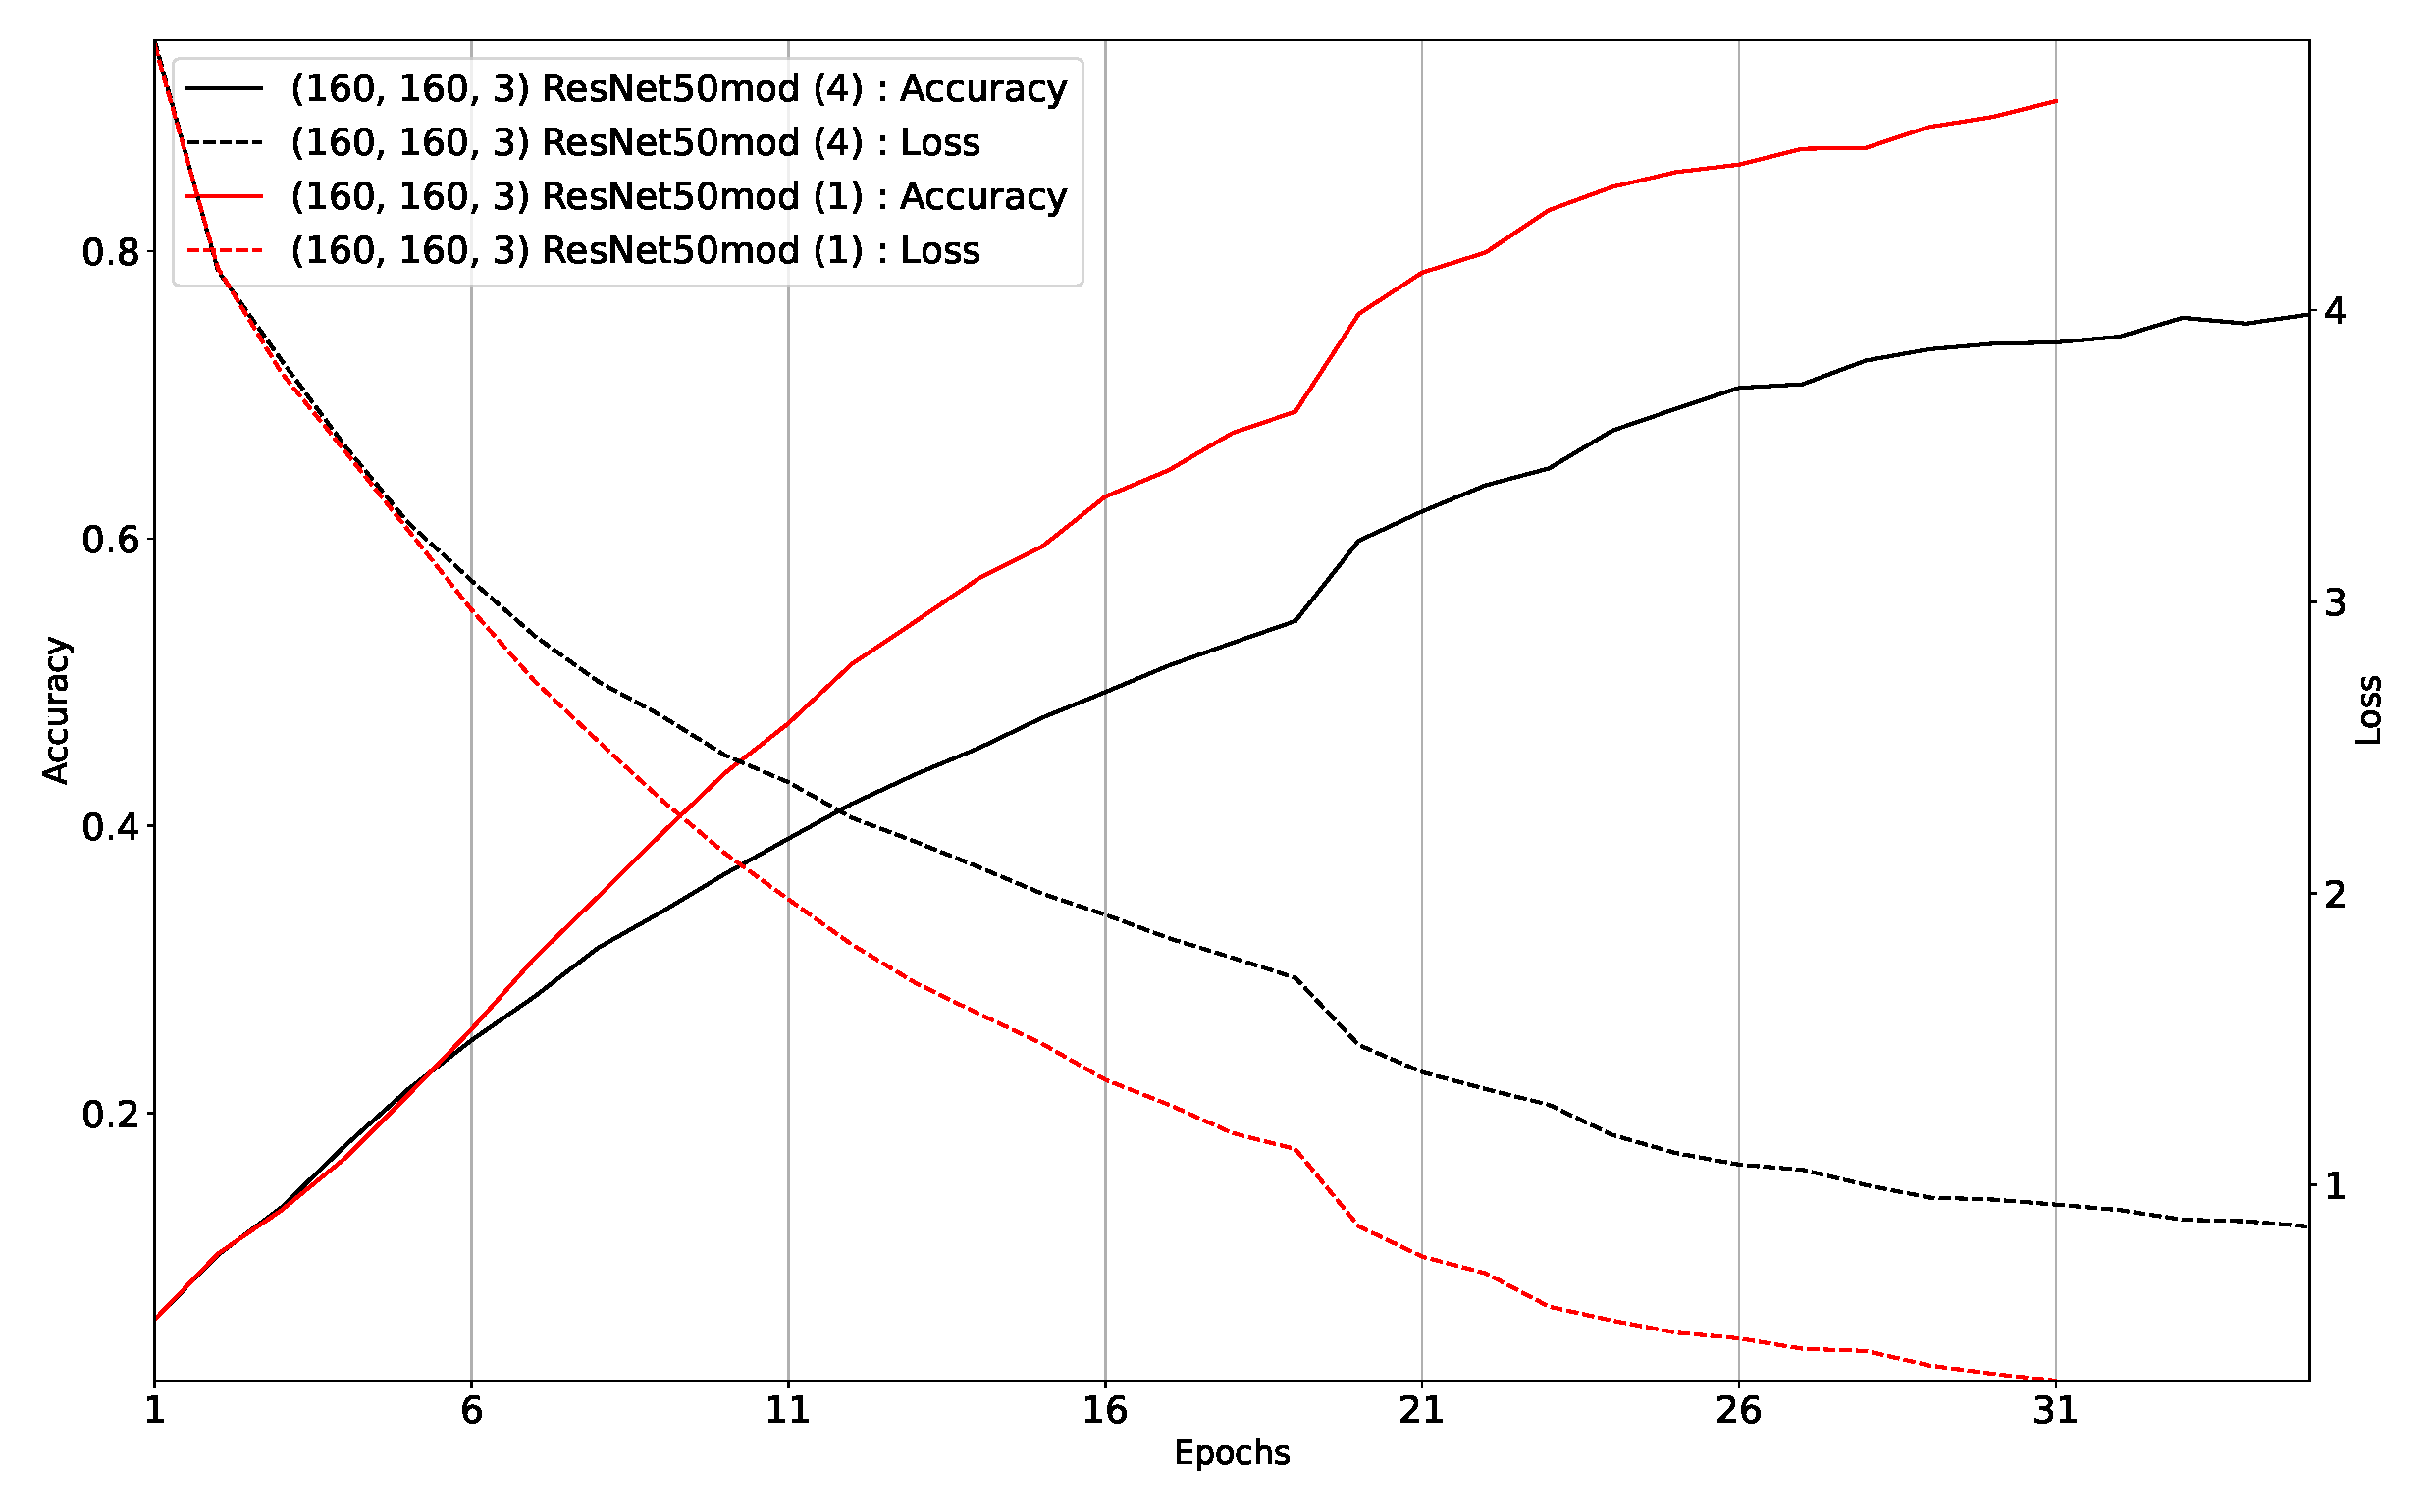
\includegraphics[width=\textwidth]{History_Compare_20unfrozen_0unfrozen_Training.pdf}
\caption{Training}
\label{image_unfrozen20_training}
\end{subfigure}
\begin{subfigure}[t]{0.49\textwidth}
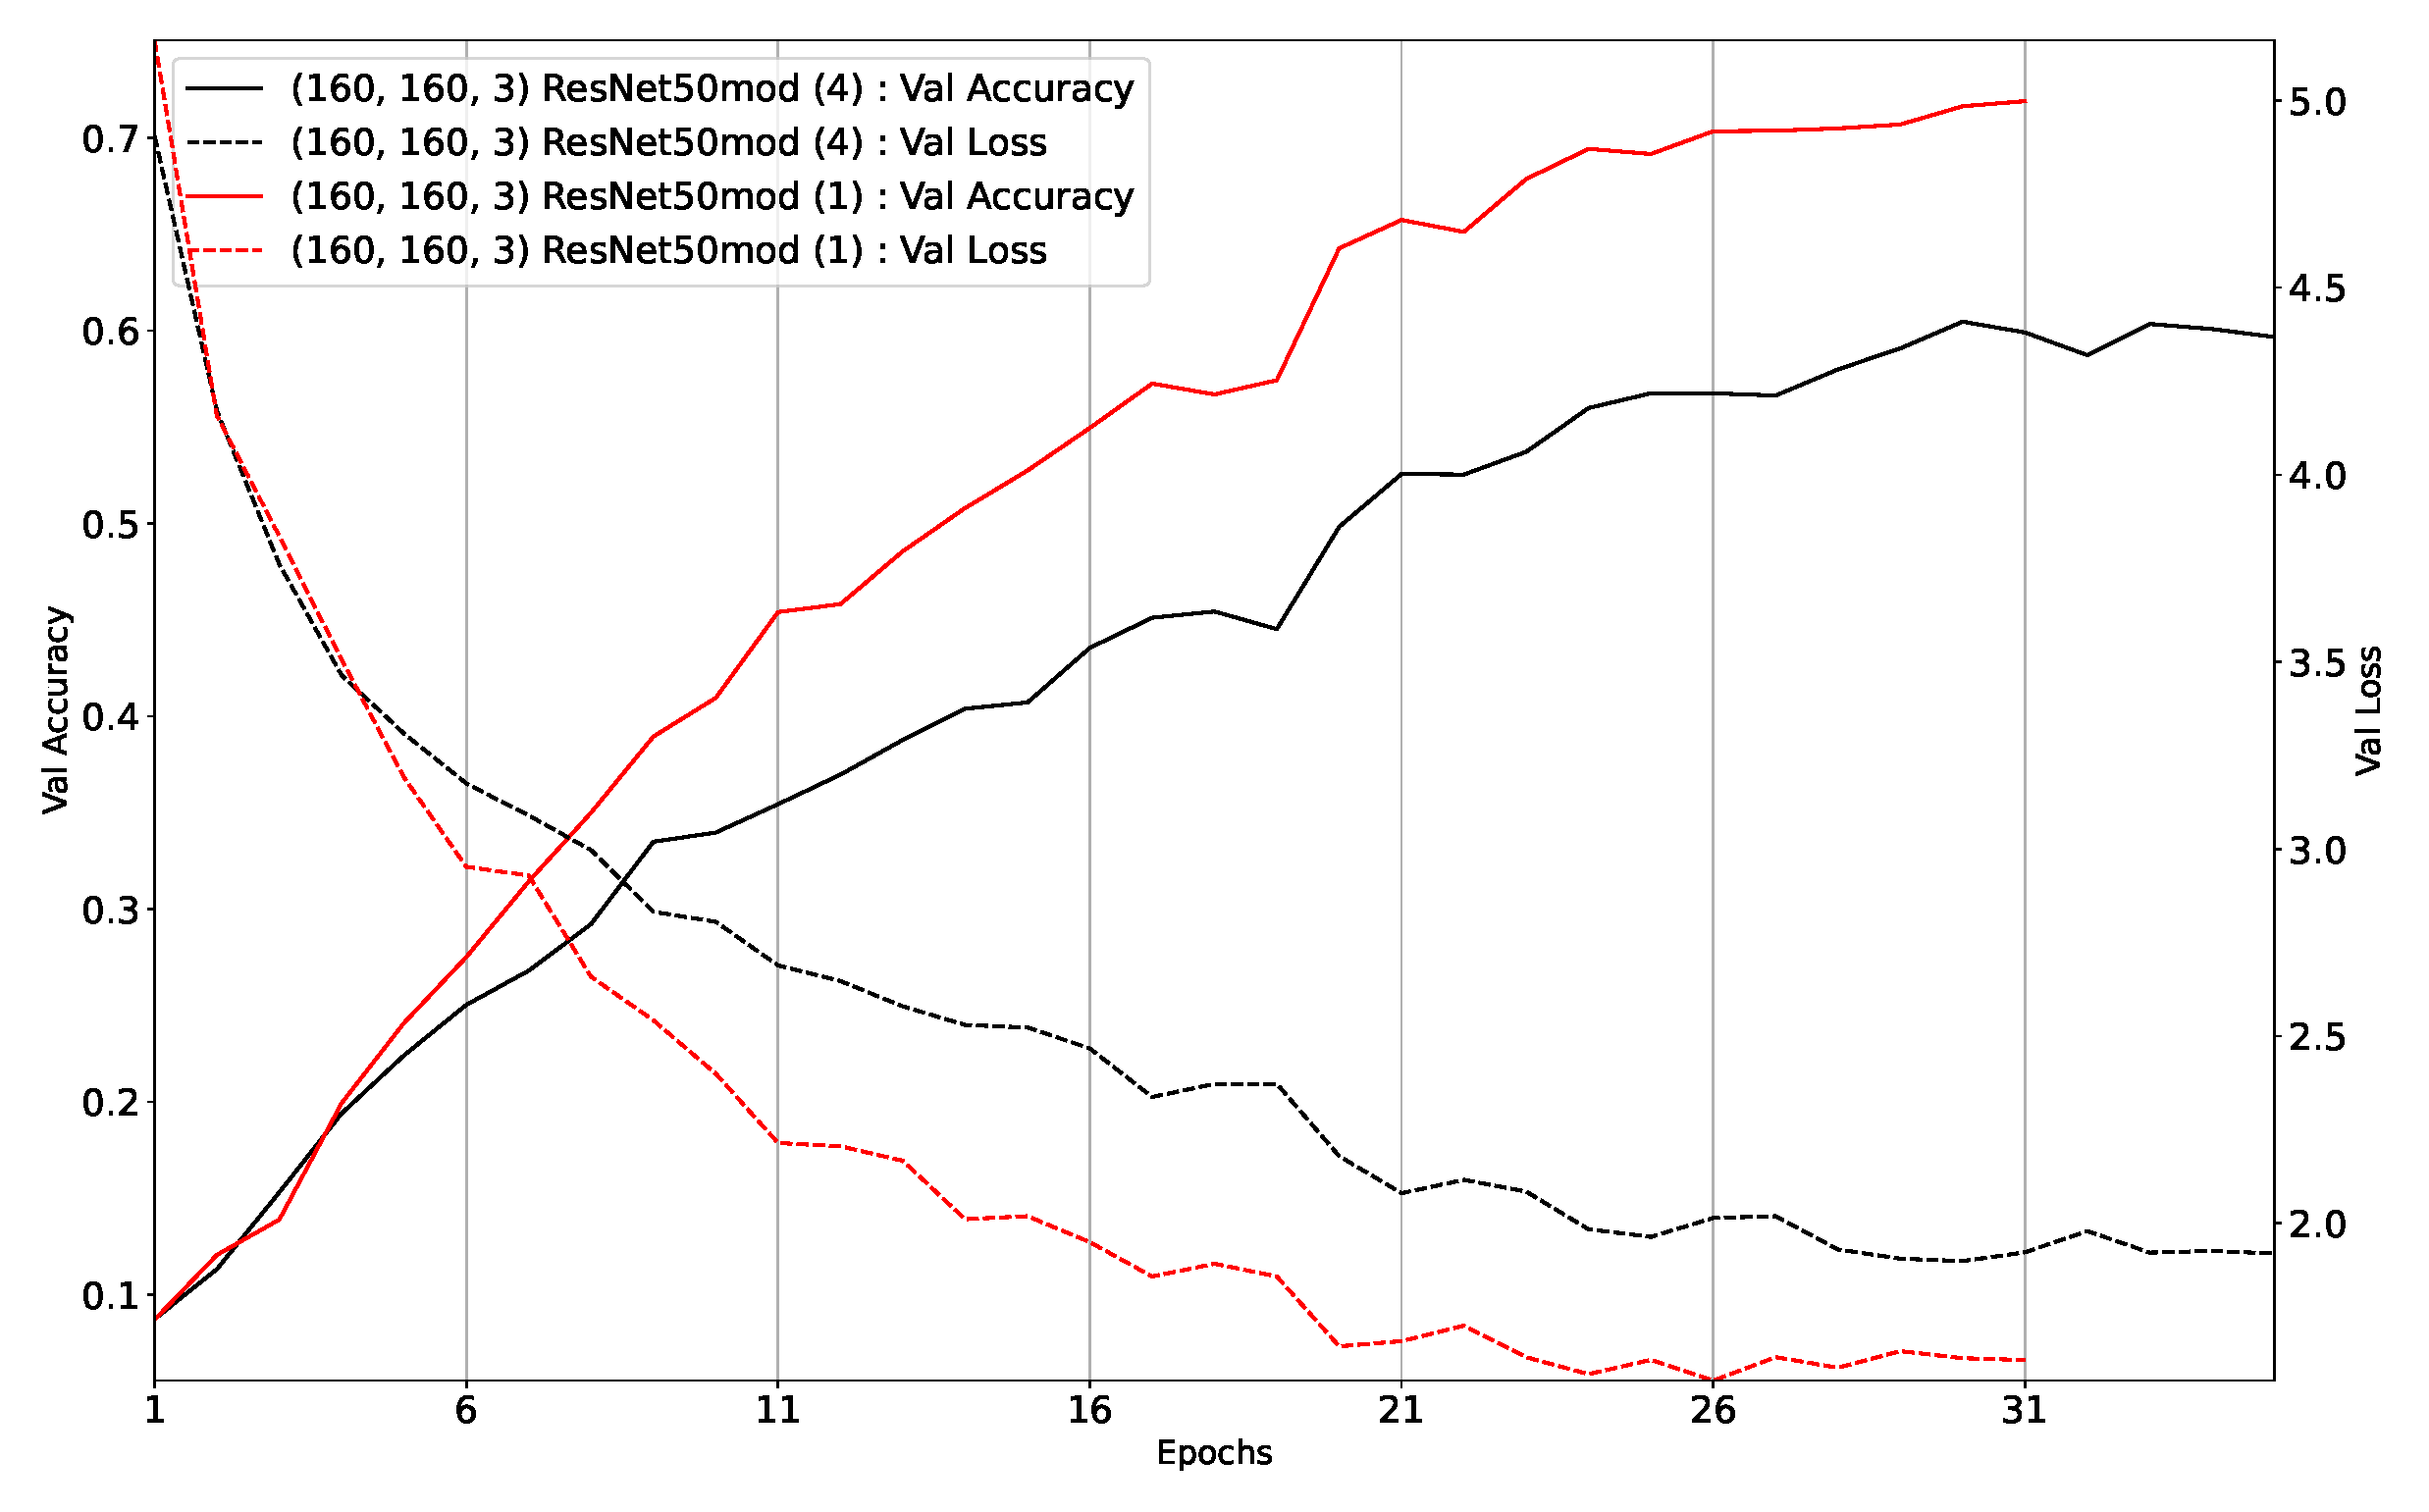
\includegraphics[width=\textwidth]{History_Compare_20unfrozen_0unfrozen_Validation.pdf}
\caption{Validation}
\label{image_unfrozen0_validation}
\end{subfigure}
\caption{Επίδραση ξεπαγώματος επιπέδων}
\label{Unfreeze_Layers_fig}
\end{figure}

\subsection{Επιλογή αρχιτεκτονικής}
\label{Architecture Selection}
Στις προηγούμενες παραγράφους παρουσιάστηκε η επίδραση που είχε στην εκπαίδευση μιας συγκεκριμένης αρχιτεκτονικής ένα πλήθος παραμέτρων όπως το μέγεθος των εικόνων, η χρήση image generator, καθώς και οι αποφάσεις που λήφθηκαν βασιζόμενοι σε αυτές τις δοκιμές. Η υπόθεση που έγινε ήταν ότι η συμπεριφορά που επιδείχθηκε στο τροποποιημένο μοντέλο ResNet50 θα ήταν ίδια και στα υπόλοιπα μοντέλα.

Έχοντας καταλήξει λοιπόν στο ποιο είναι το καταλληλότερο ResNet50mod παρουσιάζουμε στο σχήμα \ref{Training_History_Train} την εξέλιξη των τιμών ακρίβειας και της συνάρτησης κόστους για πέντε μοντέλα. Όπως γίνεται αντιληπτό το μοντέλο με την μεγαλύτερη ακρίβεια είναι το ResNet50mod για εικόνες (256, 256, 3) το οποίο και θα χρησιμοποιήσουμε στο επόμενο βήμα της εργασίας της μεταφοράς μάθησης. 


%\begin{figure}[H]
%\centering
%\begin{subfigure}[t]{1.0\textwidth}%
%\includegraphics[width=\textwidth]{History_Training.pdf}
%\end{subfigure}
%\caption{Ιστορία Εκπαίδευσης}
%\label{Training_History_Train}
%\end{figure}

\begin{figure}[H]
\centering
\begin{subfigure}[t]{1.0\textwidth}
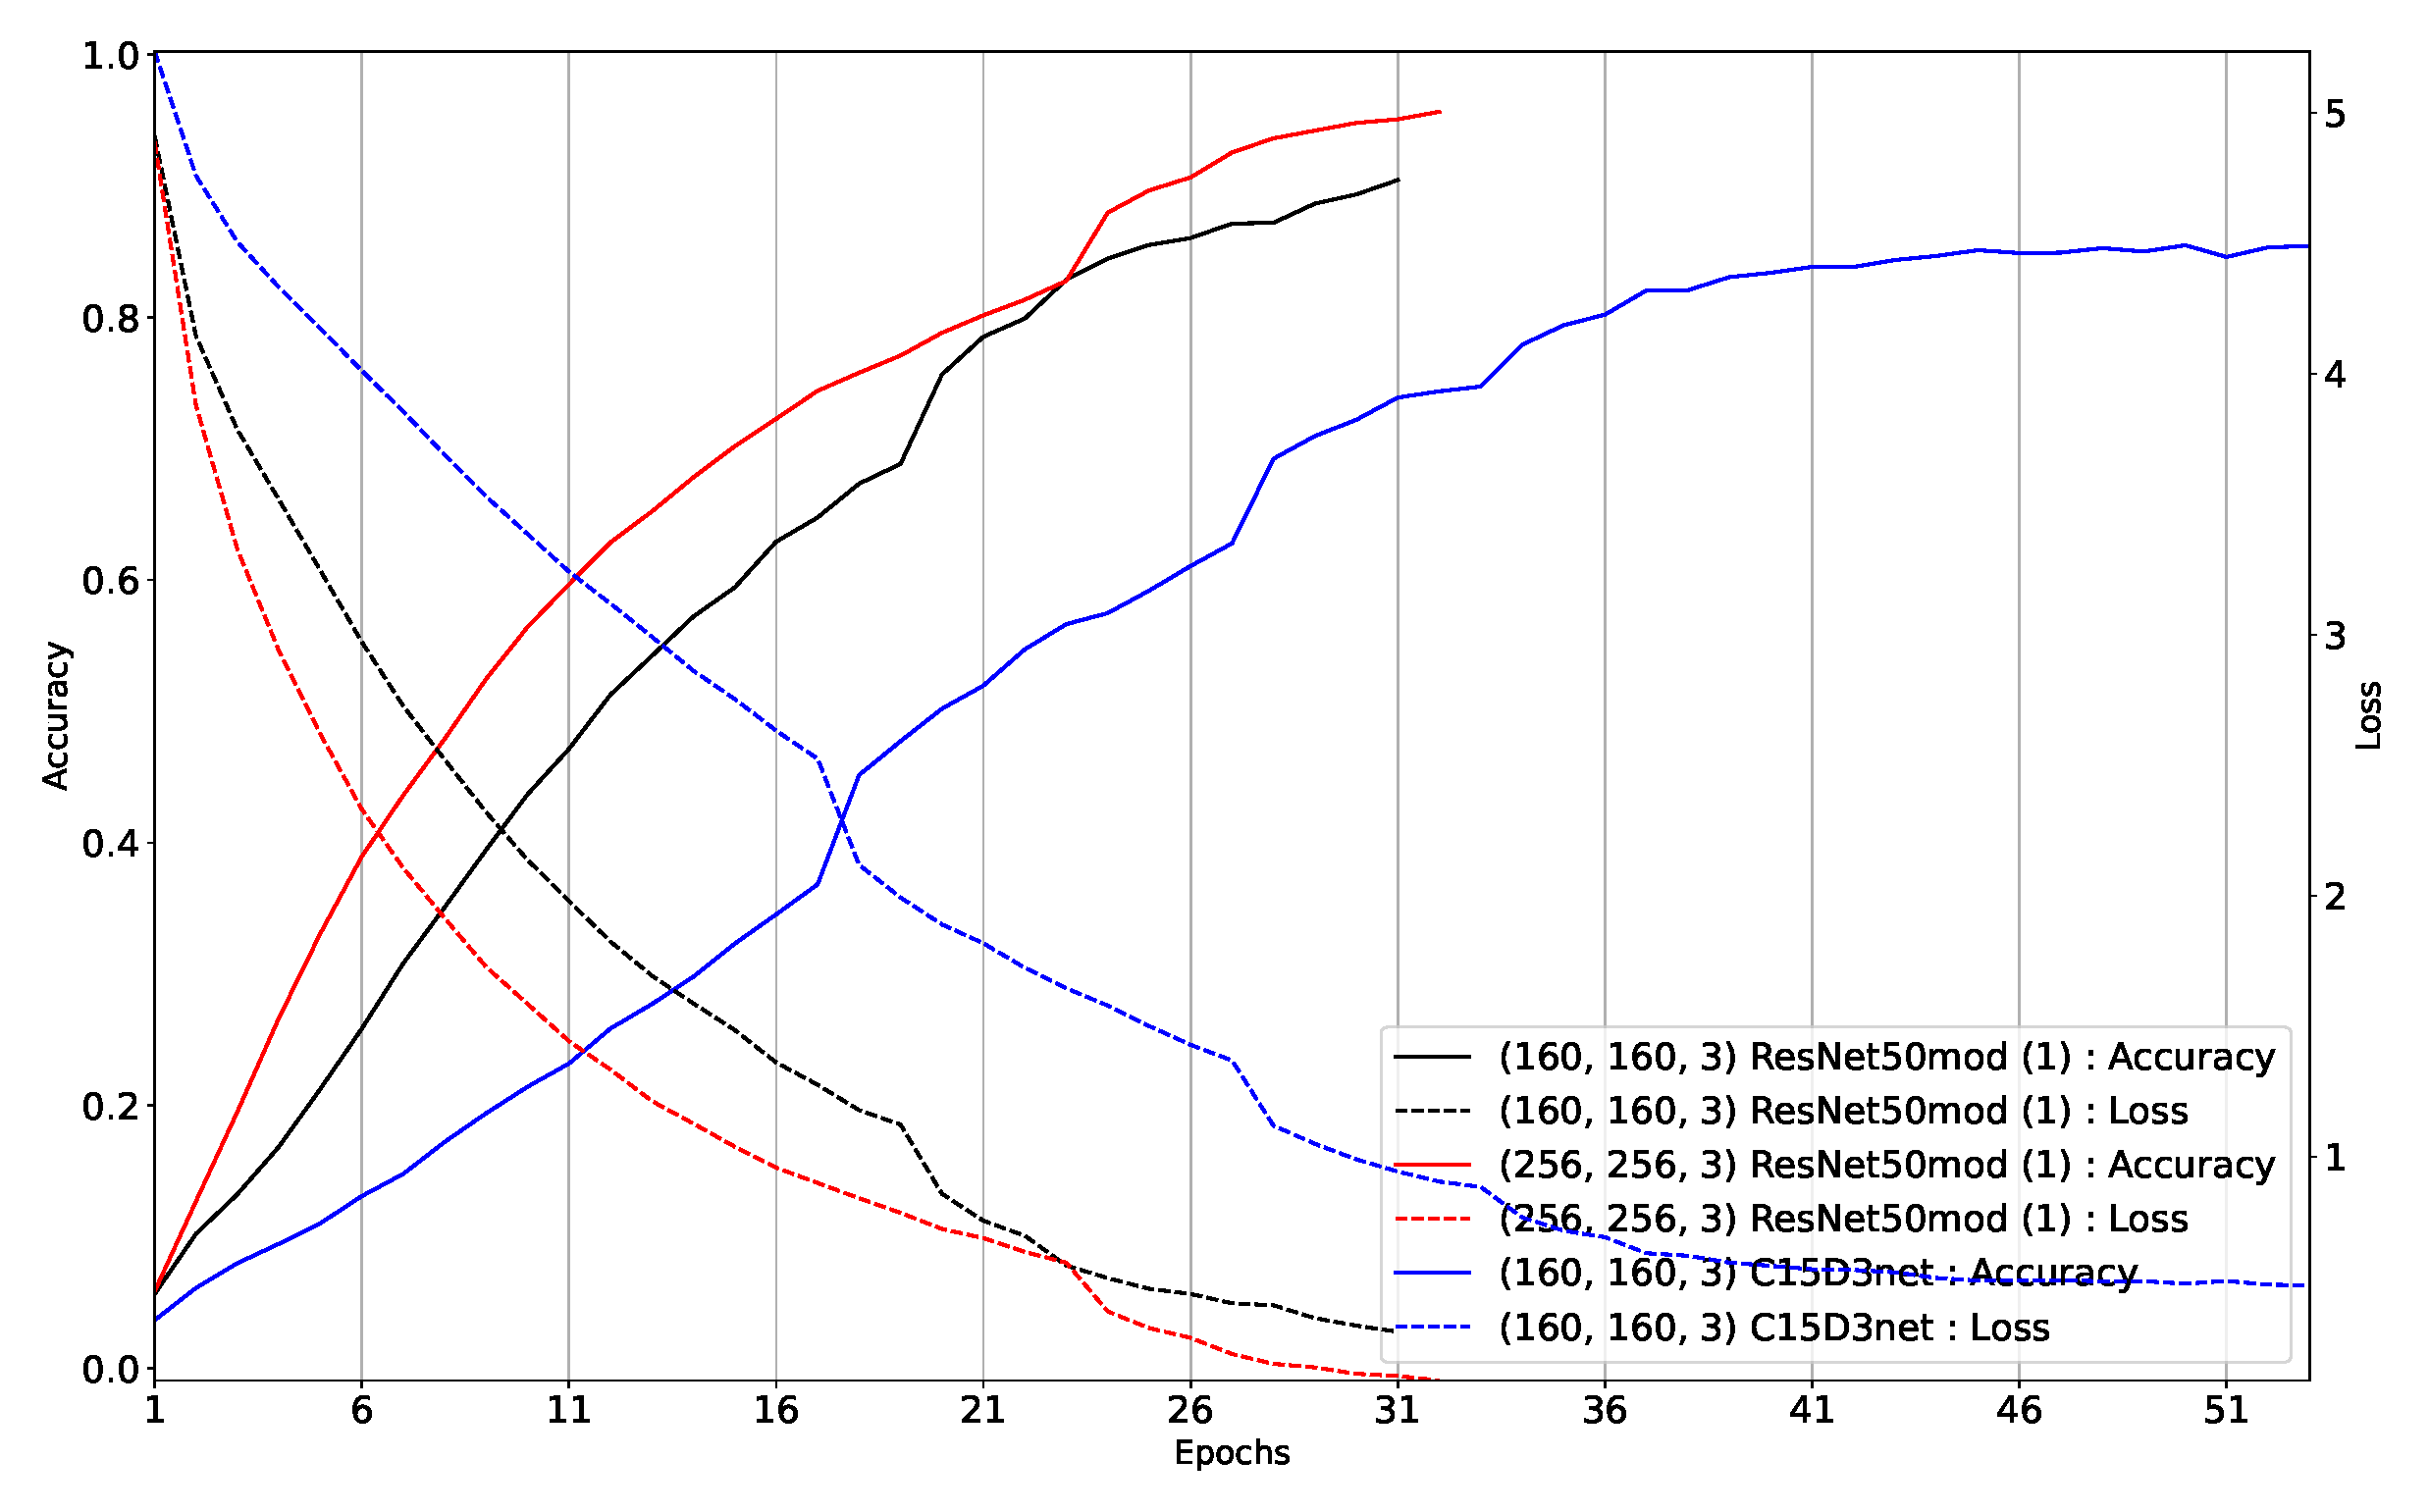
\includegraphics[width=\textwidth]{History_Compare_Models_160_Training.pdf}
\caption{Training}
\label{image_unfrozen20_training}
\end{subfigure}
\begin{subfigure}[t]{1.0\textwidth}
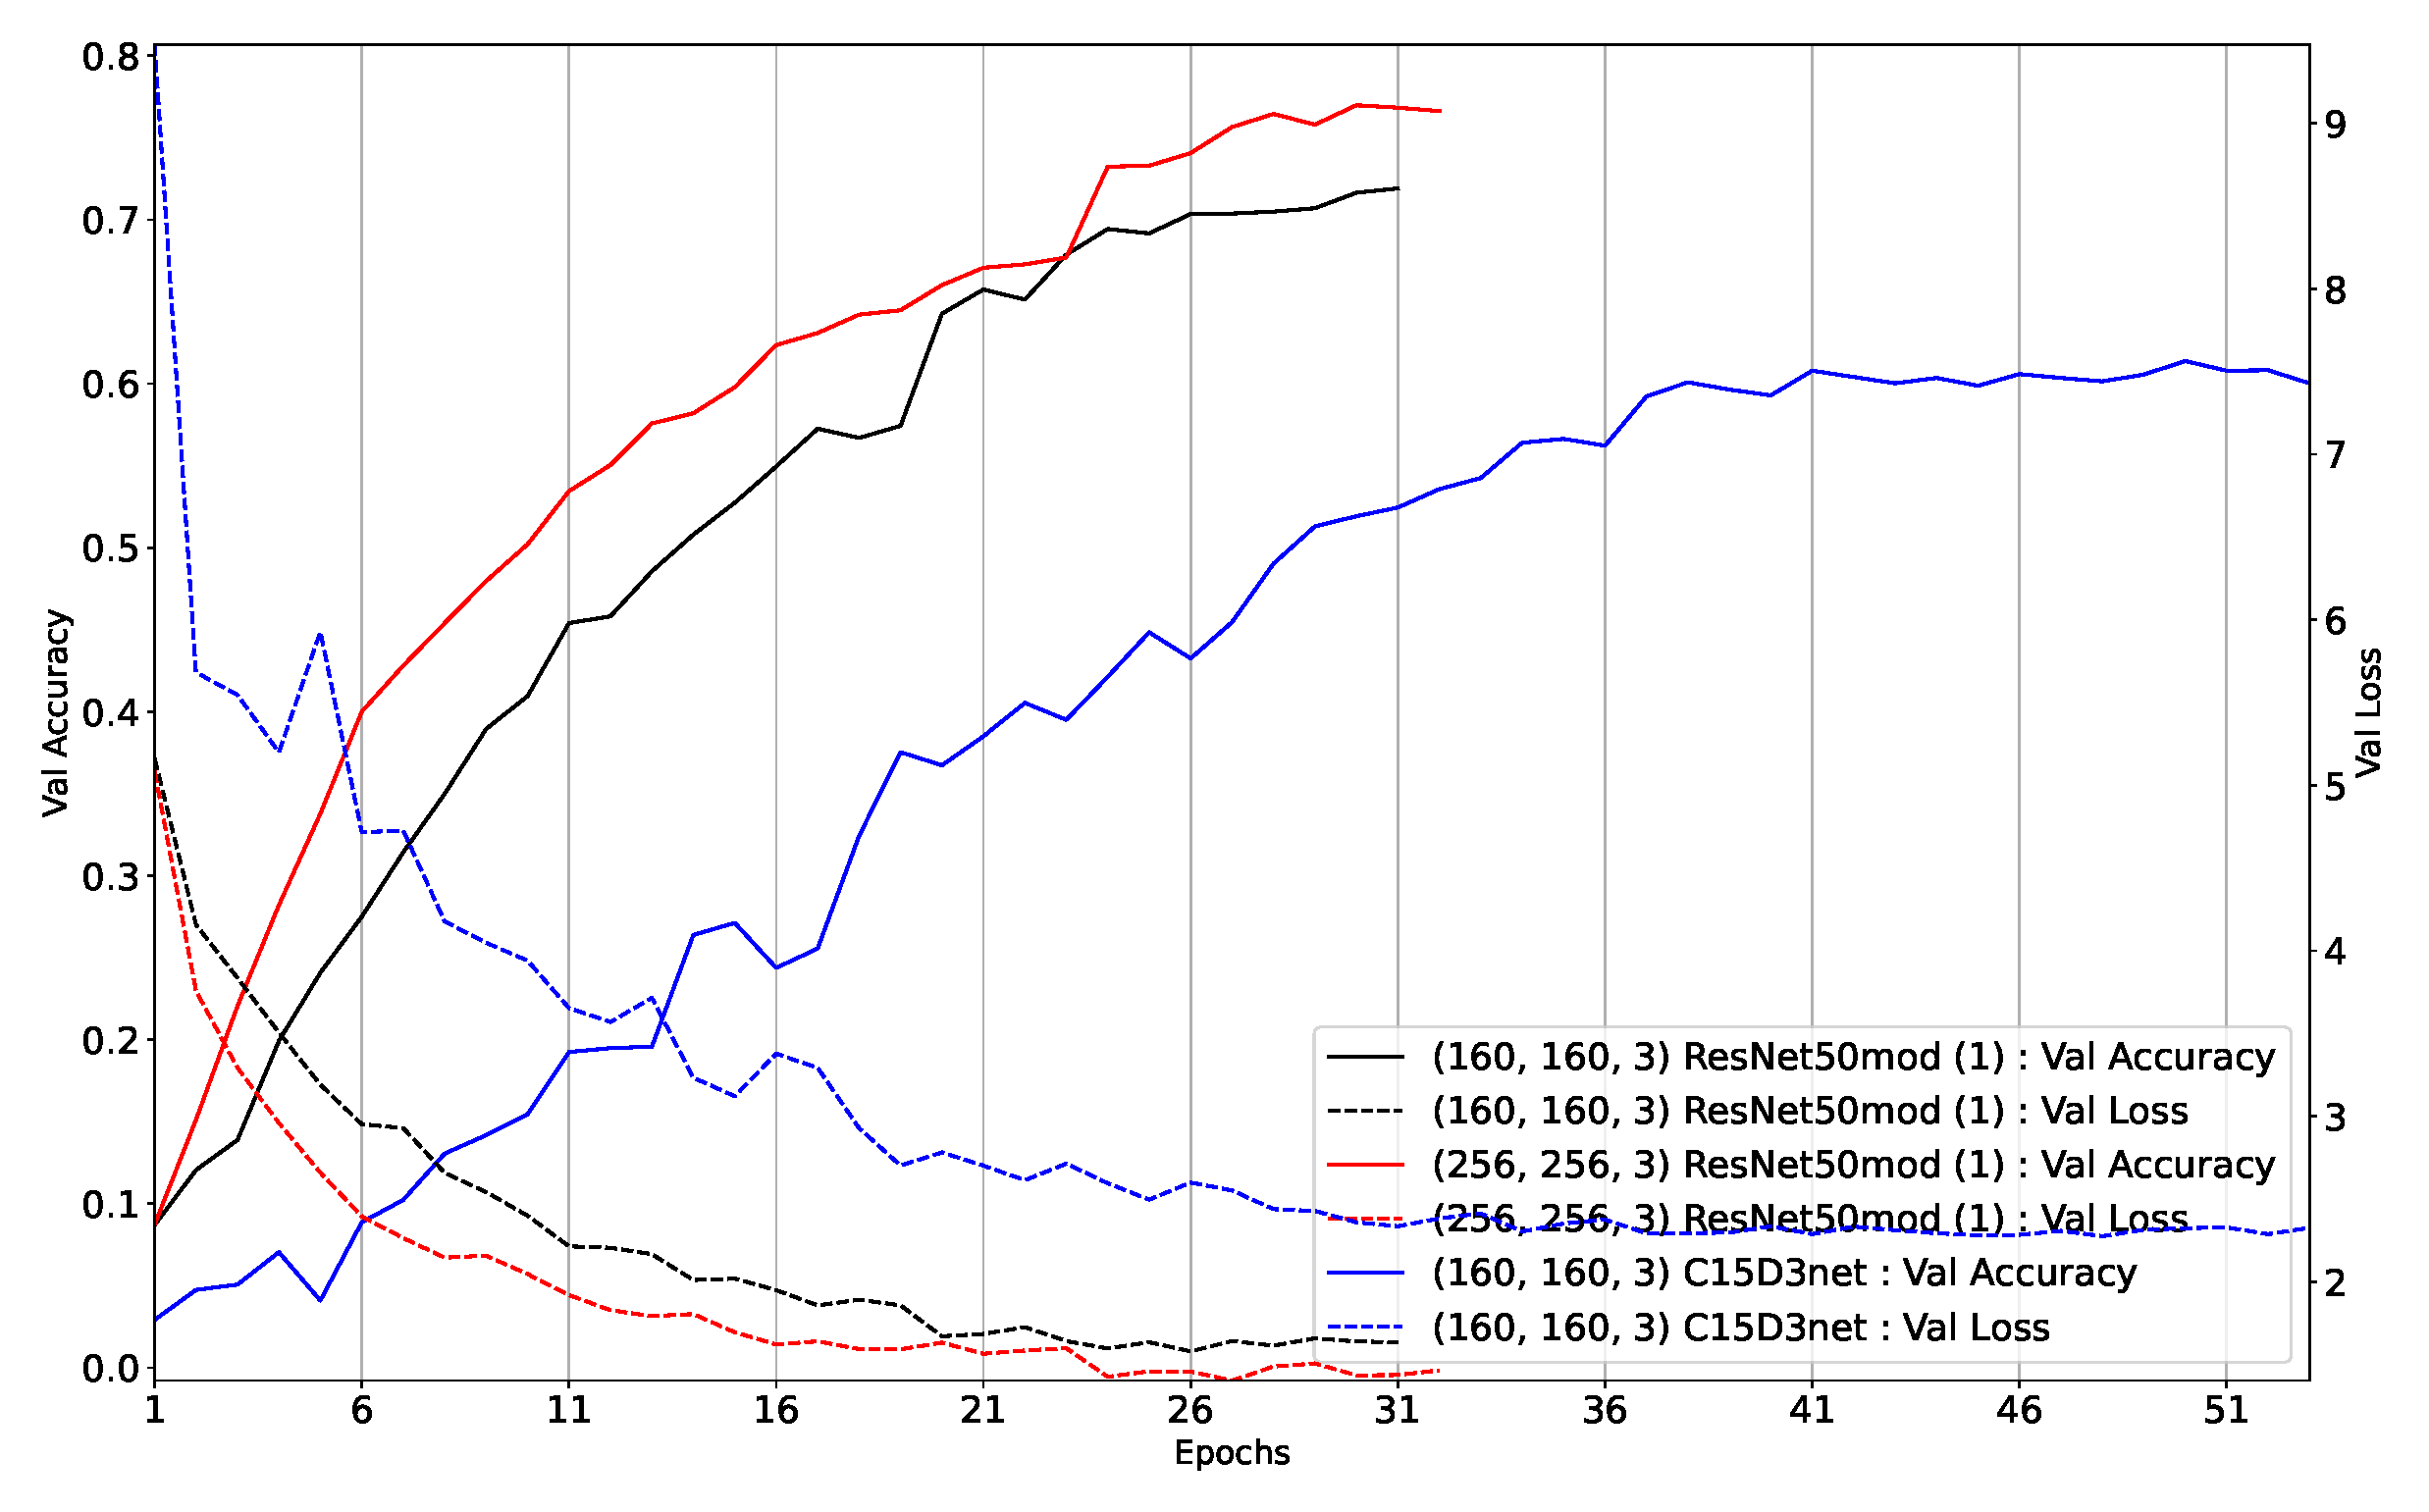
\includegraphics[width=\textwidth]{History_Compare_Models_160_Validation.pdf}
\caption{Validation}
\label{image_unfrozen0_validation}
\end{subfigure}
\caption{Ιστορία Εκπαίδευσης}
\label{Training_History_Train}
\end{figure}